\documentclass[9pt,twocolumn,twoside]{pnas-new}

% Use the lineno option to display guide line numbers if required.
% Note that the use of elements such as single-column equations
% may affect the guide line number alignment. 
\templatetype{pnasresearcharticle} 

% Choose template 
% {pnasresearcharticle} = Template for a two-column research article
% {pnasmathematics} = Template for a one-column mathematics article
% {pnasinvited} = Template for a PNAS invited submission
\usepackage{amsthm} 
\usepackage{amsmath} 
\usepackage{amssymb} 
\usepackage{multicol} 
\usepackage{array}
\usepackage{hyperref}

\DeclareMathOperator*{\argmax}{argmax} 
\newtheorem{axiom}{Axiom} 
\newtheorem{theorem}{Theorem}
\newtheorem{conjecture}{Conjecture} 

% \title{Curiosity is an optimal solution to the exploration-exploitation dilemma}
\title{A curiosity trick can solve all explore-exploit problems.}

\author[a,b,1]{Erik J Peterson} 
\author[a,b,c,d]{Timothy D Verstynen} 
\affil[a]{Department of Psychology} 
\affil[b]{Center for the Neural Basis of Cognition} 
\affil[c]{Carnegie Mellon Neuroscience Institute}
\affil[d]{Biomedical Engineering, Carnegie Mellon University, Pittsburgh PA}
\leadauthor{Peterson} 
\authordeclaration{The authors have no conflicts of interest to declare.}

% \equalauthors{\textsuperscript{1}A.O.(Author One) and A.T. (Author Two) contributed equally to this work (remove if not applicable).}
\correspondingauthor{\textsuperscript{1}To whom correspondence should be addressed. E-mail: Erik.Exists@gmail.com}

% --------------------------------------------------------------------
\begin{abstract}
    Explore-exploit problems are a common but intractable problems in reward learning, and therefore in the biological sciences. In this paper, we provide an alternative view of these problems that does not depend on exploring to optimize for reward value, even though this remains the goal of exploitation. Here exploration has no objective but learning itself which we equate to curiosity. Through theory and experiments we show this ``curiosity trick'' leads to optimal value solutions for potentially all explore-exploit problems, if that is curiosity is just as important as reward collection for survival. In particular, we show our approach succeeds in naturalistic conditions when rewards are sparse, deceptive, and non-stationary. We also suggest three experiments that might be used to distinguish our approach from other theories.
\end{abstract}
    
% SIGNIFICANCE
\significancestatement{
An animal exploring a new environment quickly finds itself with a difficult question: Is it better to keep exploring, or exploit and stick with the known? This problem, the explore-explto aalloit dilemma, is mathematically intractable but common to all animals. When one mathematical problem can’t be solved, it’s often good to find another related problem that can be. In this work we show that when exploration is re-imagined as an open-ended search to learn as much as possible, curiosity, it becomes possible find simple tracatable solutions for all explore-exploit problems, if that is curiosity is just as important as reward for long-term survival. 
}
% \dates{This manuscript was compiled on \today}
% \doi{\url{www.pnas.org/cgi/doi/10.1073/pnas.XXXXXXXXXX}}
\begin{document} 
\verticaladjustment{-2pt} 
\maketitle

\thispagestyle{firststyle} \ifthenelse{\boolean{shortarticle}}{\ifthenelse{\boolean{singlecolumn}}{\abscontentformatted}{\abscontent}}{}

% TODO: the search for reward depends on having a good world model. This is not made clear. Such limits are not discussed... enough? Fix this during revision!
% \section*{Introduction}

% --------------------------------------------------------------------
% Input the rest

%  TODO - Need oprn-field/maze cites with no reward
Exploration behavior can have two very different explanations depending on whether an animal might receive a reward. If there is no reason to expect a reward, exploration is treated as a search for information. For example, when a rat is placed in a novel environment it will explore even if no food and water is expected \cite{Berlyne1950}. We equate this with curiosity \cite{Berlyne1950,Schmidhuber1991,Kidd2015,Jaegle2019,Sumner2019,Wang2019,Auersperg2015}. If reward is expected however exploration is interpreted as a search for reward \cite{Gupta2006,Sutton2018,Woodgate2017,Lee2011a,Schulz2018a,Calhoun2014}.

An open problem in the decision sciences is to unify exploration with exploitation, which we define as the policy of choosing the most rewarding action. This union is known to be difficult and the conflict between them leads to the famous exploration-exploitation dilemma \citep{Kelly1956,Berger-Tal2014,Dayan1996,Thrun1992,Mehlhorn2015,Kobayashi2019}. We illustrate this classic paradox in Fig. \ref{fig:bee}a.

In this paper, we show that exploration is better handled by an information search, even when the goal is to collect the most reward. We can justify our use of curiosity because it is already known to be a primary drive in most, if not all, animals \cite{Berlyne1950,Loewenstein1994,Inglis2001}. It is as strong, if not sometimes stronger, than the drive for reward \cite{Loewenstein1994,Kidd2015,Gottlieb2018,Sumner2019,Gopnik2020,Song2019,Wang2019}. We illustrate our alternative in Fig. \ref{fig:bee}b.

\begin{figure}
	\begin{fullwidth}
	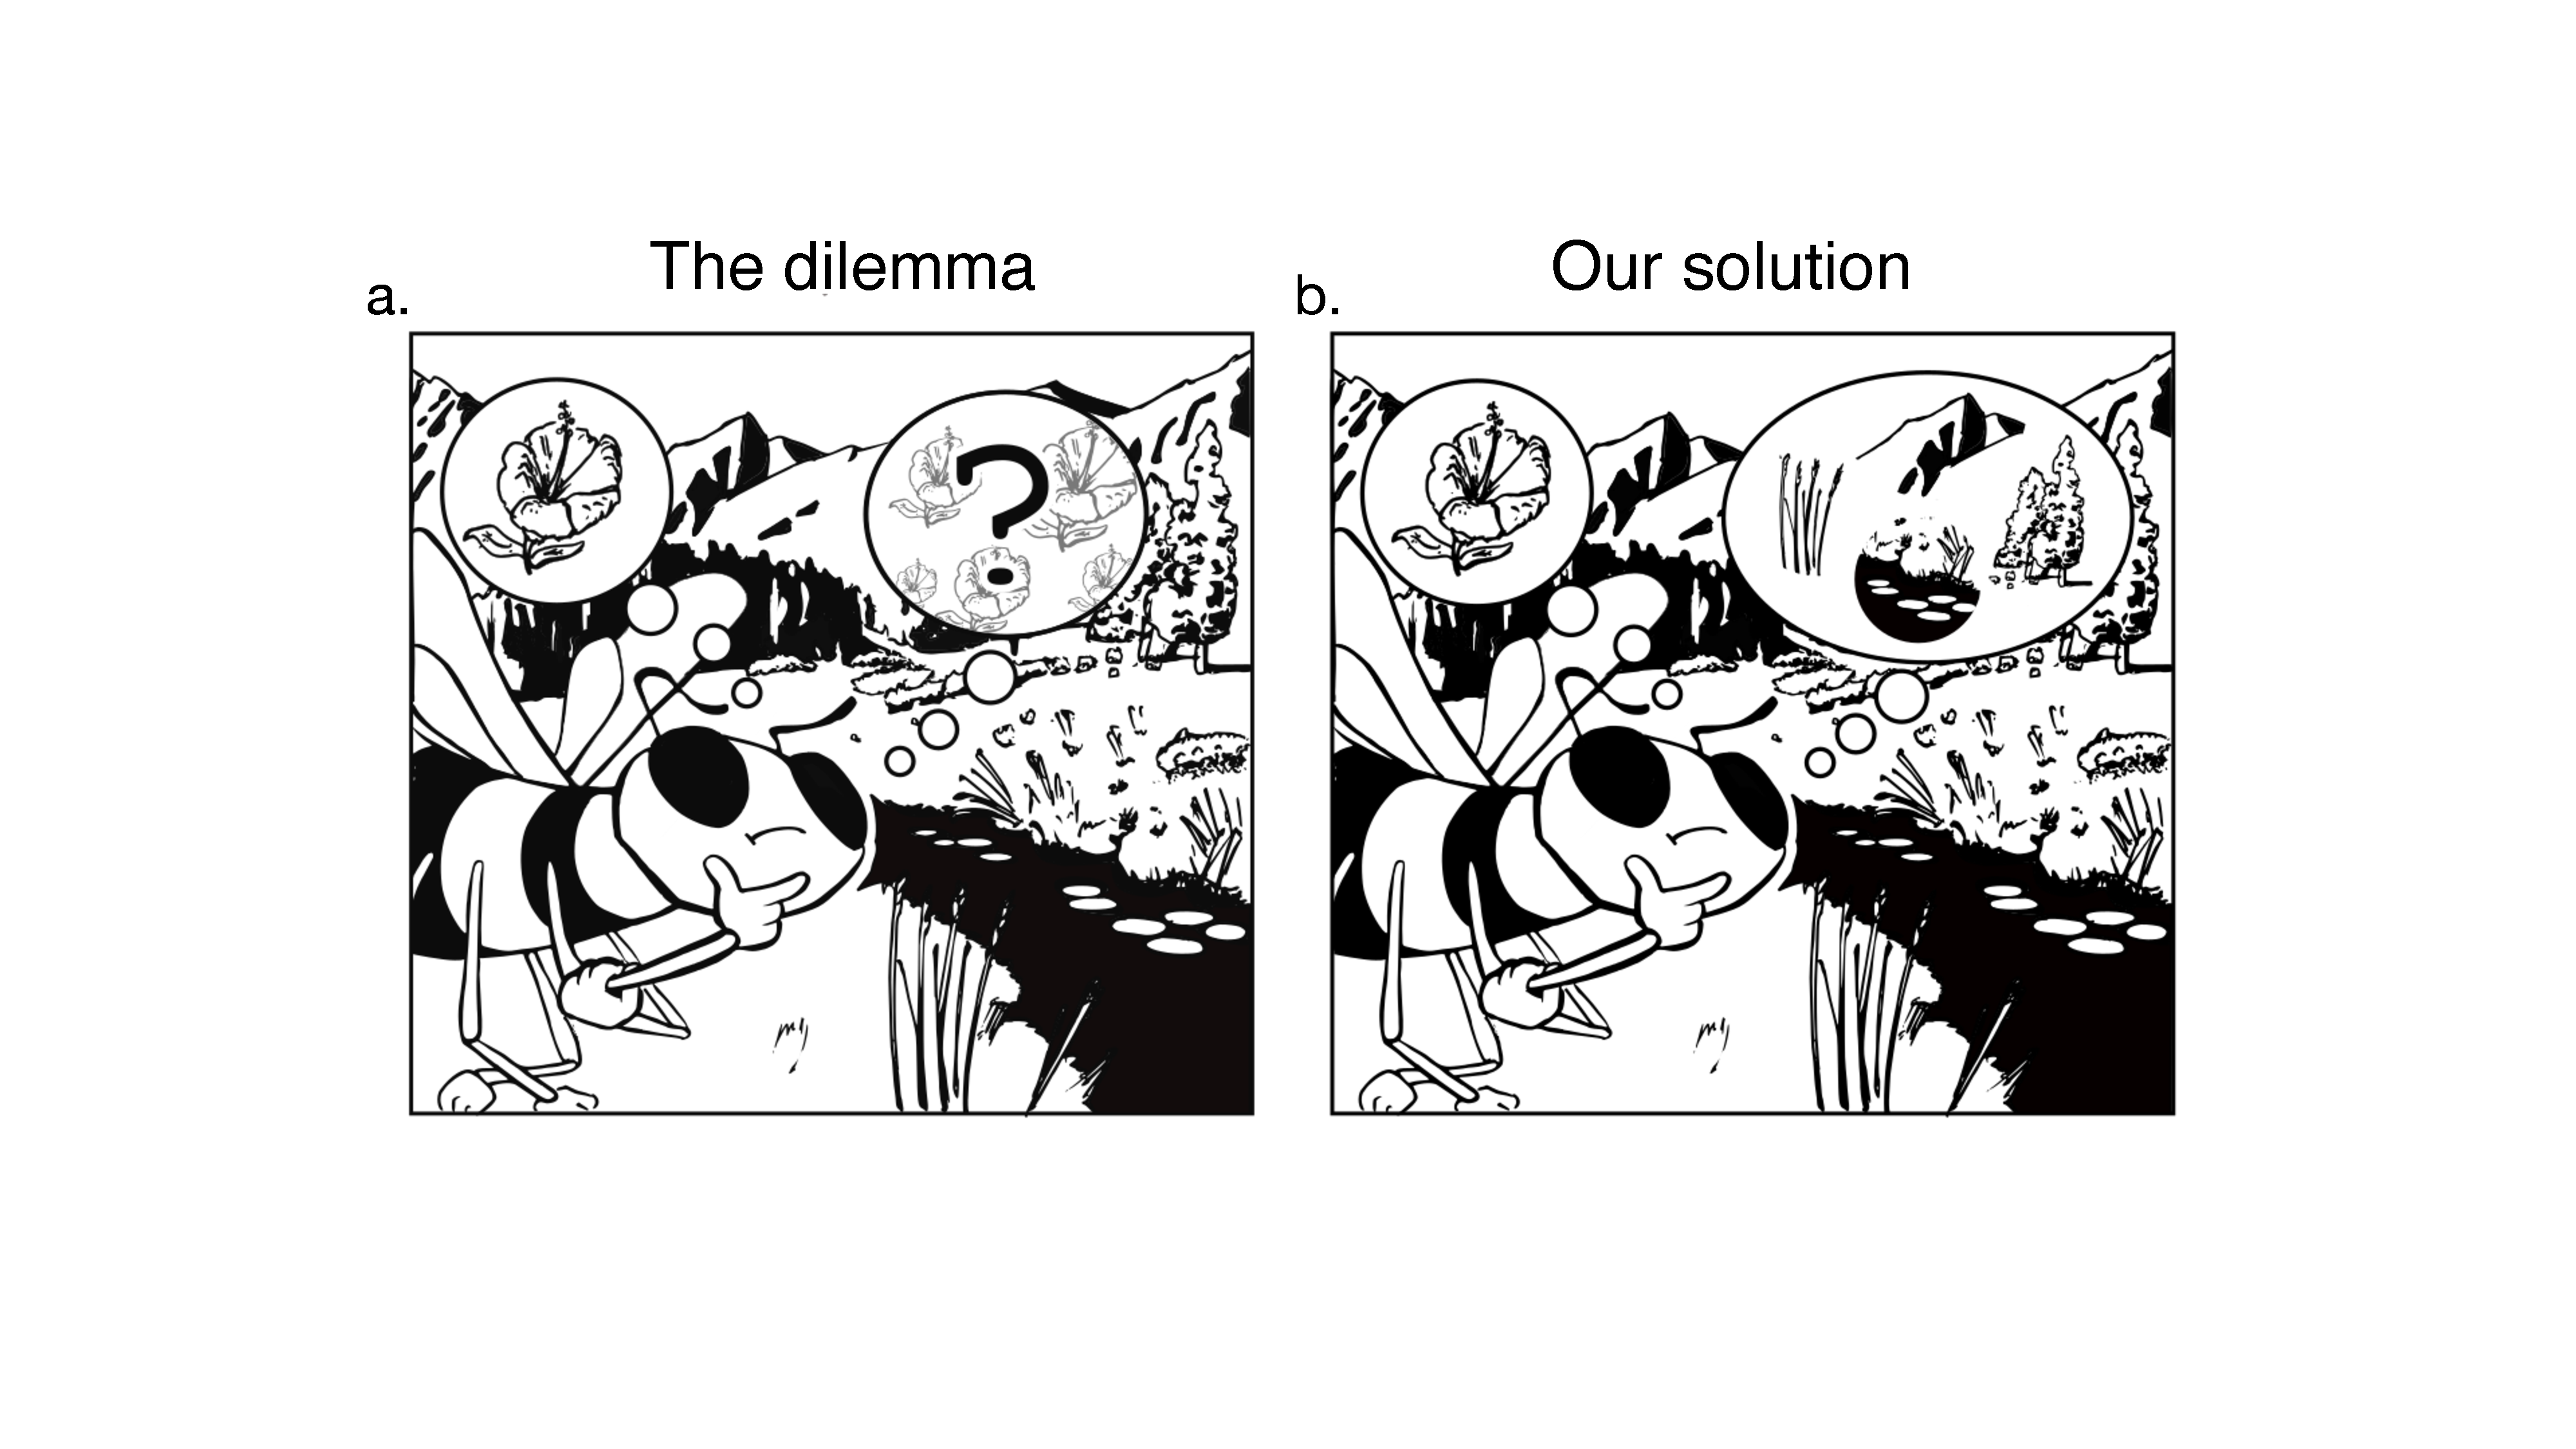
\includegraphics[width=.55\linewidth]{img/bee.pdf} 
	\caption{Two views of exploration and exploitation. \textbf{a}. The dilemma: either exploit an action with a known reward (e.g., return to the previous flower) or explore other actions on the chance they will return a better outcome. The central challenge here is that the outcome of exploration is uncertain, and filled with questions. \textbf{b}. An alternative view of the dilemma, with two goals: either maximize rewards \textit{or} maximize information value,s with a curious search of the environment. \textit{Artist credit}: Richard Grant.}
	\label{fig:bee} 
	\end{fullwidth}
\end{figure}

If exploration is just a search for information, then what was the dilemma can be divided into two problems. One problem is exploration (recast as a curious search). The other is exploitation, which still means a search for max reward. The focus of this paper is deriving a greedy and deterministic algorithm for solving both problems, simultaneously. We first develop a new mathematical view of information value, curiosity, and a new understanding of ideal curious search. The second half uses these first results to prove our curiosity trick leads to an optimal value solution for nearly all explore-exploit decisions.

% When we observe an animal grappling with the decision to either explore or exploit, we often imagine this decision is based on reward. For example, if a bee goes in a familiar direction \textit{to gather nectar}, it is said to be exploiting past knowledge for environmental reward. If it goes in an unfamiliar direction \textit{to gather nectar}, it is said to be exploring for reward. Because the environment is partly unkown to the bee, it cannot rationally choose which action it should be doing, exploiting or exploring \textit{to gain more reward}. It is this uncertainty \textit{about returning the most rewards} that makes explore-exploit choices a dilemma. It is also this uncertainty which ensures there is no tractable mathematical solution for explore-exploit questions about reward \citep{Thrun1992a,Dayan1996,Ishii2002,Simsek2006,Gershman2018b}. We illustrate this view in Fig. \ref{fig:bee}a.

% The choice between exploring and exploiting is indeed faced routinely by learners of all kinds, including foraging bees, business organizations, humans, worms, monkeys, rodents, birds, children, and computer algorithms \citep{Gupta2006,Sutton2018,Woodgate2017,Lee2011a,Schulz2018a,Calhoun2014,Wang2019,Sumner2019,Auersperg2015}. But is reward really fundamental to it? Because in the natural world exploration already finds two explanations. If there is no reason to expect a reward, exploration is described theoretically as a search for information, what we will call curiosity \citep{Berlyne1950,Schmidhuber1991,Kidd2015,deAbril2018,Jaegle2019}. On the other hand, if reward is expected, then exploration gets re-interpreted as we described above, as a search for reward, and this specific interpretation is what leads the famous dilemma \citep{Kelly1956,Berger-Tal2014,Dayan1996,Thrun1992,Mehlhorn2015,Kobayashi2019}. 

% Why curiosity? Curiosity is a rational behavoir \cite{Rich2016a}, or so we argue. Curiousity is just as important for survival as reward collection \cite{Thrun1992}. Curiosity is a primary drive in most, if not all, animals \cite{Inglis2001}. It is as strong, if not sometimes stronger, than the drive for reward \cite{Loewenstein1994,Kidd2015,Gottlieb2018}. Curiosity, as an algorithm, is highly effective at solving optimization problems \cite{Schmidhuber1991,Pathak2017,Stanton2018,Lehman201,Mouret2011b1,Fister2019,Mouret2015,Colas2020,Cully2015,Pathak2017,Schwartenbeck2019.Laversanne-Finot2018}. In short, curiosity is necesssary, omnipresent, and effective.
\section*{Results} 
\subsection*{Theory}
For our theoretical work, we first introduce reinforcement learning, and its basis in the Bellman equation. Next we develop a new mathematical view of information value, curiosity, and a new understanding of ideal curious search. We then use these results to argue that exploration-for-curiosity leads to optimal value solutions for all explore-exploit problems, with deterministic dynamics.


\subsubsection*{The reward collection problem}
Here we consider an animal who interacts with an environment over a sequence of states, actions and rewards. The animal's goal is to select actions in a way that maximizes the total reward collected. How should an animal do this? 

When the environment is unknown, to maximize reward an animal must trade-off between exploration, and exploitation. The standard way of approaching this tradeoff is to assume, 

\begin{quote}
The agent must try a variety of actions and progressively favor those that appear to be best'' \cite{Sutton2018}. 
\end{quote}

A convenient way to study reward collection is with using Markov decisions.
Our Markov decision process (MDP) for reward collection consists of states of real valued vectors $\mathbf{S}$ from a finite set $\mathcal{S}$ of size $n$, as are actions $\mathbf{A}$ from a finite set $\mathcal{A}$ of size $k$. Rewards are non-negative real numbers, $R$. Transitions from state to state are handled by the transition function $\Lambda(\mathbf{S},\mathbf{A})$. In our mathematics we assume $\Lambda$ is a deterministic function of its inputs. In our simulated experiments we assume it is a stochastic function.

Markovian preliminaries in place, we can write down the standard value function definition, and the standard Bellman equation \cite{Bellmann1954} for reward collection \cite{Sutton2018}. For simplicity we assume below that the horizon is finite, bounded by $T$.

\begin{equation} 
	\label{eq:bellman_seq}
    \begin{split}
        V^*_{R}(\mathbf{S}) &= \argmax_{\mathbf{A} \in \mathbb{A}} \Big [\sum_{k=0}^{T}  R \ \Big ]\\
                         	&= \argmax_{\mathbf{A} \in \mathbb{A}} \Big [ R_{t} + \sum_{k=0}^{T} R_{t+1} \ | \ \mathbf{S_t} = \mathbf{S},\ \mathbf{A_t} = \mathbf{A} \Big ]\\
							&= \argmax_{\mathbf{A} \in \mathbb{A}} \Big [ R_{t} + V^*_{R}(\mathbf{S_{t+1}}) \ | \ \mathbf{S_t} = \mathbf{S},\ \mathbf{A_t} = \mathbf{A} \Big ]\\
                         	&= R_0 + V^*_{R}(\mathbf{S_{t}}) + V^*_{R}(\mathbf{S_{t+1}}),\ \ldots
    \end{split}
\end{equation}

The second to last equation is the optimal Bellman equation for $V^*_R$. This can be restated more compactly as,

\begin{equation} 
\label{eq:bellman_iter}
V^*_R(\mathbf{S}) = \argmax_{\mathbf{A} \in \mathbb{A}} \Big [ R_{t}  + V^*_{R}(\Lambda(\mathbf{S},\mathbf{A})) \Big ]
\end{equation}

Having this last equation means a central challenge in reinforcement learning is efficiently estimating $V^*_{R}(.)$. This includes finding good approximate learning rules. For example, temporal difference learning or Q learning \cite{Sutton2018}. It also includes finding good exploration methods, which is of course the problem we take up here. In our eventual union, we assume the learning rule can be any nearly reinforcement learning algorithm. 


\subsubsection*{Formal regret}
Regret minimization is a standard metric of optimality in reinforcement learning \cite{Sutton2018}. Regret compares the best value response, to the chosen one. Formally, given \emph{any} any optimal value solution we can define regret $G_t$ in terms of this, given by $G = V^* - V_t$ where $V_t$ is the value of the chosen action $\mathbf{A}_t$. An optimal value algorithm can then be restated, as a ``best'' series of best actions ($\mathbf{A}_t$, $\mathbf{A}_{t+1}$, $\mathbf{A}_{t+2}$, ...) for which $\sum_{k=0}^{T} G_t = 0$.

\subsubsection*{The information collection problem}
Imagine we wish to arrive at an equation to maximize curious behavior, in terms of information value. Assume, as a stand-in, $\hat E$ represents the information value of some observation. This hypothetical equation we want could be written to match Eq.~\ref{eq:bellman_iter}. As, 

\begin{equation} 
	\label{eq:bellman_iter_E}
	V^*_{\hat E}(\mathbf{S}) = \argmax_{\mathbf{A} \in \mathbb{A}} \Big [ \hat E_{t}  + V^*_{\hat E}(\Lambda(\mathbf{S},\mathbf{A})) \Big ]
\end{equation}

We add a ``hat'' to this term $E$ to indicate it is a subject value. In constrast $R$, the external reward define about, has no ``hat''. Until, that is, we dicuss homeostatic reward value $\hat R$ later on. 

So how can we arrive at Eq.~\ref{eq:bellman_iter}? How can we ensure $\hat E$ is general, and therefore suitable for use across species? How can we do so when we choose to limit ourselves to non-Markovian kinds of learning and memory? 


\emph{Observations.} Animals at different stages in development, and in different environments, express curious behavior about the environment, their own actions, and their own mental processes. We assume a parsimonious way to handle this is be assuming curious animals often ``bind'' \cite{Robertson2003} the elements of environment, the Markov process ($\mathbf{S},\mathbf{A},\mathbf{S'},R$), into single observations $\mathbf{X}$. For convenience, we assume observations are embedded in a finite real space, $\mathbf{X} \in \mathcal{X}$ of size $l$. This binding is imagined to happen via a communication channel, $T$, identical to our observation function, $T(\mathbf{S},\mathbf{A},\mathbf{S'},R,\mathbf{M})$. ($\mathbf{M}$ is the animal's memory, that we define below.)

Observations made by $T$ can be internally generated from memory $\mathbf{M}$, or externally generated from the environment ($\mathbf{S}$,$\mathbf{S'}$). Or both can be used in combination, as happens in recurrent neural circuits. Observations may contain action information $\mathbf{A}$, but this is optional. Observations may contain reward information $R$, but this optional. Though omitting reward would hamper solving explore-exploit problems. 

\emph{Memory.} Sustained firing, the strength between two synapses, elevated Calcium concentration are three simple examples of learning and memory in the nervous system. Each of these examples though can be represented into a vector space. In fact, most any memory system can be so defined. 

We define memory as a set of real valued numbers, embedded in a finite space that is closed and bounded with $p$ dimensions. A learning function is then any function $f$ that maps observations $\mathbf{X}$ into memory $\mathbf{M}$. This $f$ is considered to be a valid learning function as long as the mapping changes $\mathbf{M}$ some small amount. A non-constant mapping, in other words. Using recursive notation, this kind of learning is denoted by $\mathbf{M} \leftarrow f(\mathbf{X},\mathbf{M}) $. Though we will sometimes use $\mathbf{M'}$ to denote the updated memory in place of the recursion. Other times we will add subscripts, like ($\mathbf{M}_t,\mathbf{M}_{t+1},\ldots$), to express the path of a memory. We can also define a forgetting function that \textit{can be any function} that inverts the memory, $f^{-1}(\mathbf{X};\ \mathbf{M}') \rightarrow \mathbf{M}$. 

We do not assume memory $\mathbf{M}$, or the learning function $f$ are Markovian.

For individual animals we assume $f$ and $f^{-1}$ have been chosen by evolution and experience to be learnable, efficient, and have sufficiently useful inductive bias for their particular environment \cite{Valiant1984a,Thrun1992a}. 


\subsubsection*{Axiomatic information value} 
To make our eventual union proper, we first need to separate reward value from information value in a principled and general way. We do this axiomatically.
We reason instead that the value of any observation made by an animal depends entirely on what an animal learns by making that observation–-literally how it changes that animal's memory. This lets us sidestep a problem present in most working models of curiosity. They tend to conflate the learning rule, with curiosity itself \cite{Schmidhuber1991b,Oudeyer2018a,Burda2018,Zhang2013,deAbril2018,Zhou2020,Schwartenbeck2019,Wilson2014a,Lehman2011,Velez2014}.

Our definition of information value closely follows the motivations of Shannon, and his definition of a communication channel. If we have a memory $\mathbf{M}$ which has been learned by $f$ over a history of observations, $(\mathbf{X_0},\mathbf{X_1},...)$, can we measure how much value the next observation $\mathbf{X_t}$ should have? 

We think this, our hypothetical measure $\hat E$, should have certain intuitive properties:

\begin{axiom}[Axiom of Memory]
	$\hat E$ depends only on the difference $\delta \mathbf{M}$ between $\mathbf{M}$ and $\mathbf{M'}$.
\end{axiom}

That is, the value of an observation $\mathbf{X}$ depends only on how
the memory changes, by $f$. 

\begin{axiom}[Axiom of Novelty]
	$\hat E = 0$ if and only if $\delta M = 0$. 
\end{axiom}

That is, an observation that doesn’t change the memory has no value.

\begin{axiom}[Axiom of Scholarship]
	$\hat E \ge 0$.
\end{axiom}

That is, all (new) information is in principle valuable even if its consequences are later found to be negative.

\begin{axiom}[Axiom of Completeness]
	$\hat E$ should increase monotonically with the total change in memory. 
\end{axiom}

That is, there should be a one-to-one relationship between how memory changes and how information is valued.

\begin{axiom}[Axiom of Equilibrium]
	For the same observation $\hat E$ should approach 0 in finite time.
\end{axiom}

That is, learning on $\mathbf{M}$ makes continual progress toward equilibrium (i.e. self-consistency) with each observation, after a finite time period has passed. After this it will approach a steady-state value of $\delta \mathbf{M} \rightarrow 0$ and $\hat E \rightarrow 0$. We use the term consistency to denote a memory at or near equilibrium. We mean that the memory has become consitent it itseslf in time, and this all our axioms can promise. 

All we have really done in these axioms is remove any mention of a learning rule, its properties, or learning target, its properties from previous definitions \cite{Itti2009,Jaegle2019,Schmidhuber1991,Inglis2001,Reddy2016,Pirolli2007}. This is important not for its own sake but because with these axioms we can consider information value, and therefore curiosity, independent of any learning semantics, or any semantics at all. 

Put another way, if information should be agnostic to semantics \cite{Shannon1948a}, we reason information value should be agnostic as well.


\subsubsection*{Practical information value}
Meeting our requirements is not difficult. The practical example of axiomatic value we use throughout this paper is based on the geometric norm, $||.||$ (as shown in Fig.~\ref{fig:cartoon}). Though not necessarily a unique solution, a norm on the memory gradient is a simple, computational convenience, way to satisfy Axioms 1-4 (Eq \ref{eq:E_norm}). 

\begin{equation}
	\label{eq:E_norm}
	\hat E = || \ \nabla \mathbf{M} \ ||
\end{equation}

To satisfy Axiom 5 we further require memory dynamics eventually decelerate,  $\nabla^2 \mathbf{M} < 0$ for all $ t \ge T^*$. Informally, the idea here is that any notion of sensible and useful learning must converge. We take this to mean that in finite time bound, $T^*$, $\hat E$ must approach 0 (as shown in Fig.~\ref{fig:cartoon}b-c). We term this consistent learning.

In practice here we will not work with the gradient, but will use a discrete time map in its place,

\begin{equation}
	\label{eq:E_norm_discrete}
	\hat E \approx || \ f(\mathbf{M},\mathbf{X}) - \mathbf{M} \ ||
\end{equation}

\begin{figure}
	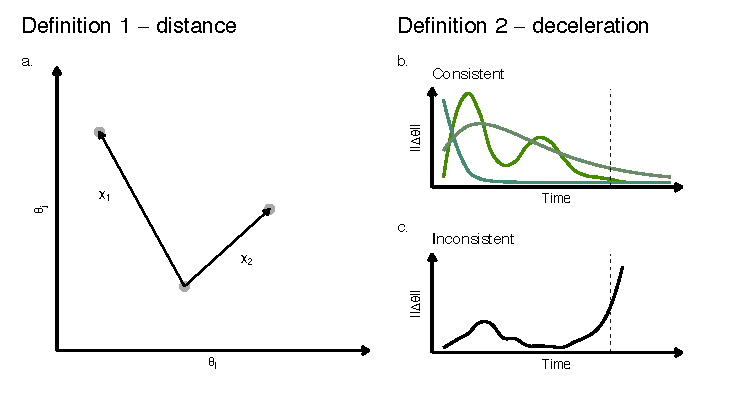
\includegraphics[width=1\linewidth]{img/cartoon.pdf} 
	\caption{Practical (geometric) information value, and our constraints on its dynamics. 
	\textbf{a}. This panel illustrates a two dimensional memory. The information value of two observations $\mathbf{X}_1$ and $\mathbf{X}_2$ depends on the norm of their memory, $\mathbf{E_1}$ and $\mathbf{E_2}$ respectively, with learning. Here we show this distance as a euclidean norm, denoted as a black arrow.
	\textbf{b-c} This panel illustrates learning dynamics with time (over a series of observations that are not shown). If information value becomes decelerating in finite time bound, then we say that learning is consistent with Def. 2. This is shown in panel b. The bound is depicted as a dotted line. If learning does not decelerate, then it is said to be inconsistent (Panel c). It is important to note that our account of information value and curiosity does not work when learning is inconsistent.
  	}
	\label{fig:cartoon} 
\end{figure}

The common way to arrive at the Bellman solution is to again assume a Markov decision space. This is a problem for our definition of memory, which we assume has a natural long-term path dependence. This breaks the Markov assumption, and its needed claim of optimal substructure. To get around this we proved that exact forgetting of the last observation is another way to achieve optimal substructure, and so to derive a Bellman solution.

In the theorem below, which shows the optimal substructure of $\mathbf{M}$, we implicitly assume that $\mathbf{X} = \mathbf{S}$, $\mathbf{A}$, $f$, and $\Lambda$ are given, and that $\Lambda$ is deterministic, 

\begin{theorem}[Optimal substructure] \label{theorem:opt_sub} 
   If $V^*_{\pi_{\hat E}}$ is the optimal information value given by policy $\pi_{\hat E}$, a memory $\mathbf{M}_t$ has optimal substructure if the last observation $X$ can be removed from $\mathbf{M}$, by $\mathbf{M-1}_{t} = f^{-1}(\mathbf{X}, \mathbf{M}_t)$ such that the resulting value $V^*_{t-1} = V^*_{t} - E_{t}$ is also optimal. 
\end{theorem}

Given an arbitrary starting value $E_0 > 0$, the best solution to maximizing $\hat E$ is can be given by a Bellman equation (Eq.~\ref{eq:bellman_iter_E}).

\begin{equation} 
	\label{eq:bellman_iter_E}
	V^*_{\hat E}(\mathbf{S}) = \argmax_{\mathbf{A} \in \mathbb{A}} \Big [ \hat E_{t}  + V^*_{\hat E}(\Lambda(\mathbf{S},\mathbf{A})) \Big ]
\end{equation}

As long as learning about the different observations $\mathbf{X}$ is independent, and as long as learning continues until steady-state, defined as $E_t < \eta$, there are many equally good solutions to the information collection problem above. Under these conditions we can therefore simplify Eq. \ref{eq:bellman_iter_E} further, giving Eq. \ref{eq:EE}. 

\begin{equation}
	\label{eq:EE} 
	V_E^{*}(\mathbf{X}) = \argmax_{\mathbf{A}} \Big [ E_t + E_{t+1} \Big ]
\end{equation}

\subsubsection*{A hypothesis about boredom}
The central failure mode of curiosity is what we will call minutia, defined as learning that has little to no use to the agent. A good example of this is to, ``Imagine a scenario where the agent is observing the movement of tree leaves in a breeze. Since it is inherently hard to model breeze, it is even harder to predict the location of each leaf'' \cite{Pathak2017}. This will imply that a curious agent will always remain curious about chaos in the leaves even though they have no hope of successful learning of them.

To limit curiosity we introduction a penalty term, $\eta$ which we treat as synonymous with boredom. We consider boredom an adaptive trait, in other words. Others have considered boredom arguing it is a useful way to motivate aversive tasks \cite{Bench2013}, or curiosity \cite{Loewenstein1994}. We take a slightly different view. We treat boredom as a tunable free parameter, $\eta \ge 0$ and a means to ignore marginal value by requiring curious exploration to stop once $E \le \eta$. 


\subsubsection*{Optimal exploration}
Having a policy $\pi_E^*$ that optimally maximizes $\hat E$ does not necessarily ensure that exploration is of good quality. We think it is reasonable to call an exploration good if it meets the criteria below. 

\begin{enumerate}
	\item Exploration should visit all available states of the environment at least once.
	\item Exploration should cease when learning has plateaued.
	\item Exploration should take as few steps as possible to achieve 1 and 2.
\end{enumerate}

In Theorems~\ref{theorem:Z} and~\ref{theorem:convergence} we prove that our Bellman solution $\pi_E$ satisfies these, when $\eta > 0$ and when the observations $\mathbf{X}$ contain complete state information, $\mathbf{S} \in \mathbf{X}$. See the Appendix for the proofs proper.

\begin{theorem}[Complete exploration] 
	\label{theorem:Z} 
	Given some arbitrary value $E_0$, an exploration policy governed by $\pi^*_{\hat E}$ will visit all states $\mathbf{S} \in \mathbb{S}$ in a finite number of steps $T$.
\end{theorem}

\begin{theorem}[Efficient exploration] 
	\label{theorem:convergence} 
	An exploration policy governed by $\pi^*_{\hat E}$ will only revisit states for where information value is marginally useful, defined by $\hat E > \eta$.  
\end{theorem}


\subsubsection*{A hypothesis of equal importance}
 Searching in an open-ended way for information must be less efficient than a direct search for reward? In answer to this question, we make two conjectures.

\begin{conjecture}[A hypothesis of equal importance]
	Reward value and information value are equally important for survival, in changing environments 
\end{conjecture}

If both reward and information are equally important, then time is not wasted in a curious search. The process is not \textit{necessarily} inefficient, or even indirect. Instead, this hypothesis leads we argue to a new question. Is curiosity practical enough to serve as a useful ``trick'' to solve all reward collection search problems? We answer this question with a second conjecture,

\begin{conjecture}[The curiosity trick]
	When learning is possible, curiosity is a sufficient solution for all exploration problems.
\end{conjecture}


\subsubsection*{The problem of mixing reward and information collection}
If reward and information are equally important, and curiosity is sufficient, how can an animal go about balancing them? If you accept our conjectures, then answering this question optimally is the same as solving the dilemma. To solve this dual value learning problem we’ve posed–-information and reward maximization–-we need an algorithm that can maximize the value of a mixed sequence, $V_{\hat{E}R}$. For example,

\begin{equation}
	\label{eq:bellman_seq_ER}
	V^*_{\hat{E}R}(\mathbf{S}) = \argmax_{\mathbf{A} \in \mathbb{A}} \Big [\sum_{k=0}^{T} \hat{E}_t + \hat{E}_{t+1} + R_{t+2} + \hat{E}_{t+3} + R_{t+4} + \ldots  \ \Big ]
\end{equation}

\subsubsection*{A win-stay, lose-switch solution}
A similar dual value optimization problem to Eq.~\ref{eq:bellman_seq_ER} was posed and solved, with its regret bounded, by Robbins \cite{Robbins1952} in his original derivation of the win-stay lose-switch rule. This WSLS approach has since proven useful in decision making and reinforcement learning \cite{Estes1994TowardAS,Worthy2014}, Bayesian sampling \cite{Bonawitz2014}, and especially in game theory \cite{Nowak1993}. We also put it to use here. 

We have come to think about our two optimal value policies $\pi_R$ and $\pi_{\hat E}$ as two ``players'' in game for behavioral control of an animal's moment-by-moment actions \cite{Estes1994TowardAS}. The simplest solution to this game, in terms of computational complexity, is a WSLS rule. We denote this rule as $\Pi_\pi$, and define it here by the inequalities below. 

\begin{equation} 
    \label{eq:pipi}
    \begin{split}
        \Pi_{\pi} = 
        \begin{cases}
            \pi^*_{\hat{E}} & : \hat{E} - \eta > R + \rho \\
            \pi_R 	& : \hat{E} - \eta < R + \rho \\
        \end{cases}
    \end{split}
\end{equation}

We assume no matter which policy is in control in Eq.~\ref{eq:pipi}, each policy can learn from (be updated using) the other policies actions, and observations. That is, while the two policies compete for control, they learn from each other in a cooperative fashion.

Here $\eta$ is the boredom term we defined earlier. We also introduce the reward bias term $\rho$, where $\rho > \eta$. This bias ensures no ties can occur, and that as $\hat E$ decreases to 0, as it must, the default policy is reward collection. That is, by $\pi_R$. In this paper we assume $\rho$ is set to be just a modest amount larger than $\eta$. Its role is then to break ties, and little else. Larger values of $\rho$ could be used to bias reward  exploitation in ``irrational'' ways.

In Eq.~\ref{eq:pipi} we compare reward $R$ and information value $\hat E$ but have not made sure they have the same ``units''. We sidestep this issue, and at the same time ensure complete exploration, as well as convergence, by limiting the expected probability of having zero reward to be, itself, non-zero. That is, $\mathbb{E}[p(R_t=0) > 0]$. For the same reasons, we also limit $E_0$, the first set of values, to be positive and non-zero, $(E_0 - \eta) > 0$. 

o provide some intuition for Eq.\ref{eq:pipi}, imagine that in the previous action an animal observed, arbitrarily, 0.7 units of information value and no reward (i.e. $R = 0$). Using our rule on the next action the animal should then choose its exploration policy $\pi^*_{\hat{E}}$. If it explored last time, this is a ``stay'' action. If not, it is a ``switch'' action. Let's then say that with this next observation, $\hat E$ decreases to 0.2 and a reward value of 1.0 is observed. Now the animals should switch its strategy for the next round, to exploit instead.

In general, if there was more reward value then information value last round ($R > \hat E$), our rule dictates an animal should choose the reward policy. If information value dominated, $R < \hat E$, then it should choose the information gathering policy.

The WSLS rule in Eq~\ref{eq:pipi} when applied to exploration-exploitation problems can guarantee three things, shown below. 

\begin{theorem}[No regret - reward value]
	\label{th:no_regret_R}
	When $\pi_R$ is in control under $\Pi_{\pi}$, all actions are zero regret in terms of $V_R$. That is, $\sum_{k=0}^{T} G = 0$.
\end{theorem}

\begin{theorem}[No regret - information value]
	\label{th:no_regret_E}
	When $\pi_{\hat E}$ is in control under $\Pi_{\pi}$, all actions are zero regret in terms of $V_{\hat E}$. That is, $\sum_{k=0}^{T} G = 0$.
\end{theorem}

\begin{theorem}[No regret - mixed values]
	\label{th:no_regret_ER}
	When either $\pi_{\hat E}$ or $\pi_R$ is in control under $\Pi_{\pi}$, all actions are zero regret in terms of $V_{\hat{E}R}$. That is, $\sum_{k=0}^{T} G = 0$.
\end{theorem}

In each of theses Theorems we assume our definitions for $\mathbf{X}$, $\mathbf{A}$, $\mathbf{M}$, $f$, $\Lambda$, and $\Pi_{\pi}$ are implicitly given, and a finite horizon $T$. Proofs for Theorems~\ref{th:no_regret_E} and~\ref{th:no_regret_ER} follow from both reinforcement learning and our definition of information optimization having a Bellman optimality. The proof for the optimality of $V_{\hat{E}R}$ (Th~\ref{th:no_regret_ER}) is provided in the Appendix. The intuition for this proof is simple that a greedy algorithm made over two Bellman solutions is itself a Bellman solution.

In Eq.~\ref{eq:pipi} we compare reward $R$ and information value $\hat E$ but have not ensured they have the same ``units'', or are comparable valuables. We sidestep this issue by limiting the probability of having zero reward to be, itself, non-zero. That is, $p(R_t=0) > 0$. We also limit $E_0$, the first set of values, to be positive and non-zero when used with boredom, $(E_0 - \eta) \geq 0$. These constraints ensure complete ``good'' exploration (defined above) which in turn ensures optimal reward learning is possible.


\subsubsection*{Homeostatic adjustments}
We have been studying cases where reward value is fixed. That is, where the environment reward $R$ is equal to its subjective value to the animal, $\hat R$. In natural behavior though the value of reward often declines as the animal reaches satiety \cite{Keramati2014,Juechems2019,Munch2020}. This is called reward homeostasis, and it is commonly formulated as a control theory problem.

The goal in a control setting is not to maximize $R$, but to minimize the difference between collected $R$ and a set point, $\bar R$ \cite{Keramati2014,Juechems2019,Munch2020}. So, in a homeostatic setting reward value is subjective, and approximated by $\hat R \approx \bar R - R$.

Fortunately, it has been shown a reward collection policy designed for one greedy reward collection, will work for homeostasis as well \cite{Keramati2014}. However, to use a form similar to our Eq. \ref{eq:pipi} with homeostatic reward value, we need to make one modification. This is shown in Eq.~\ref{eq:pipi_h}. 

\begin{equation} 
    \label{eq:pipi_h}
    \begin{split}
        \Pi_{\pi} = 
        \begin{cases}
            \pi^*_{\hat{E}} & : \hat{E} - \eta > R - \rho \\
            \pi_R 	& : \hat{E} - \eta < R - \rho \\
        \end{cases}
    \end{split}
\end{equation}

Under homeostasis ties between values in Eq. \ref{eq:pipi} should be broken in favor of exploration. Persuing reward exploitation instead, when homeostasis is satisfied and $\hat R=0$, disturbs homeostasis. Exploitation, in the control theoretic sense of homeostatis, is therefore a suboptimal result. 

% ----------------------------------------------------------------------
\subsection*{Experiments}
Does our theory work in practice? The remainder of this paper is devoted to studying our approaches performance in simulated bandit tasks. Each task was designed to either test exploration performance in a way that matches recent experimental studies, or to test the limits of curiosity. 

\subsubsection*{Information collection}
The work so far has built up the idea that the most valuable, and most efficient, curious search will come from a deterministic algorithm. That is, every step strictly maximizes $\hat E$. It is this determinism which will let us resolve the dilemma, later on. A deterministic view of exploration seems at odds with how the problem is generally viewed today, which involves searching with some amount of randomness. Whereas if our analysis is correct, randomness is not needed or desirable, as it must lead to less value and a longer search. 

We confirm and illustrate our theoretical results for curious search using a simple information foraging task (Task 1; Fig.~\ref{fig:task_outline1}). This variation of the bandit task \cite{Sutton2018} replaces rewards with information, in this case colors. On each selection, the agent sees one of two colors according to a specific probability shown in Fig. ~\ref{fig:task_payout}a. When the relative color probabilities are about even, that arm has more entropy and so more to learn and more information value. Arms that are certain to present only one color lose their informative value quickly.

The results of this simple information seeking task are shown in Figure~\ref{fig:curiosity1}. Deterministic curiosity in this task generated more information value, in less time, and with zero regret when compared against a stochastic agent using more directed random search. As our work here predicts, noise only made the search happen slower and lead to regret. Besides offering a concrete example, performance in Task 1 is a first step in showing that even though $\pi_E$'s optimality is proven for a deterministic environment, it can perform well in other settings.

\begin{figure}

	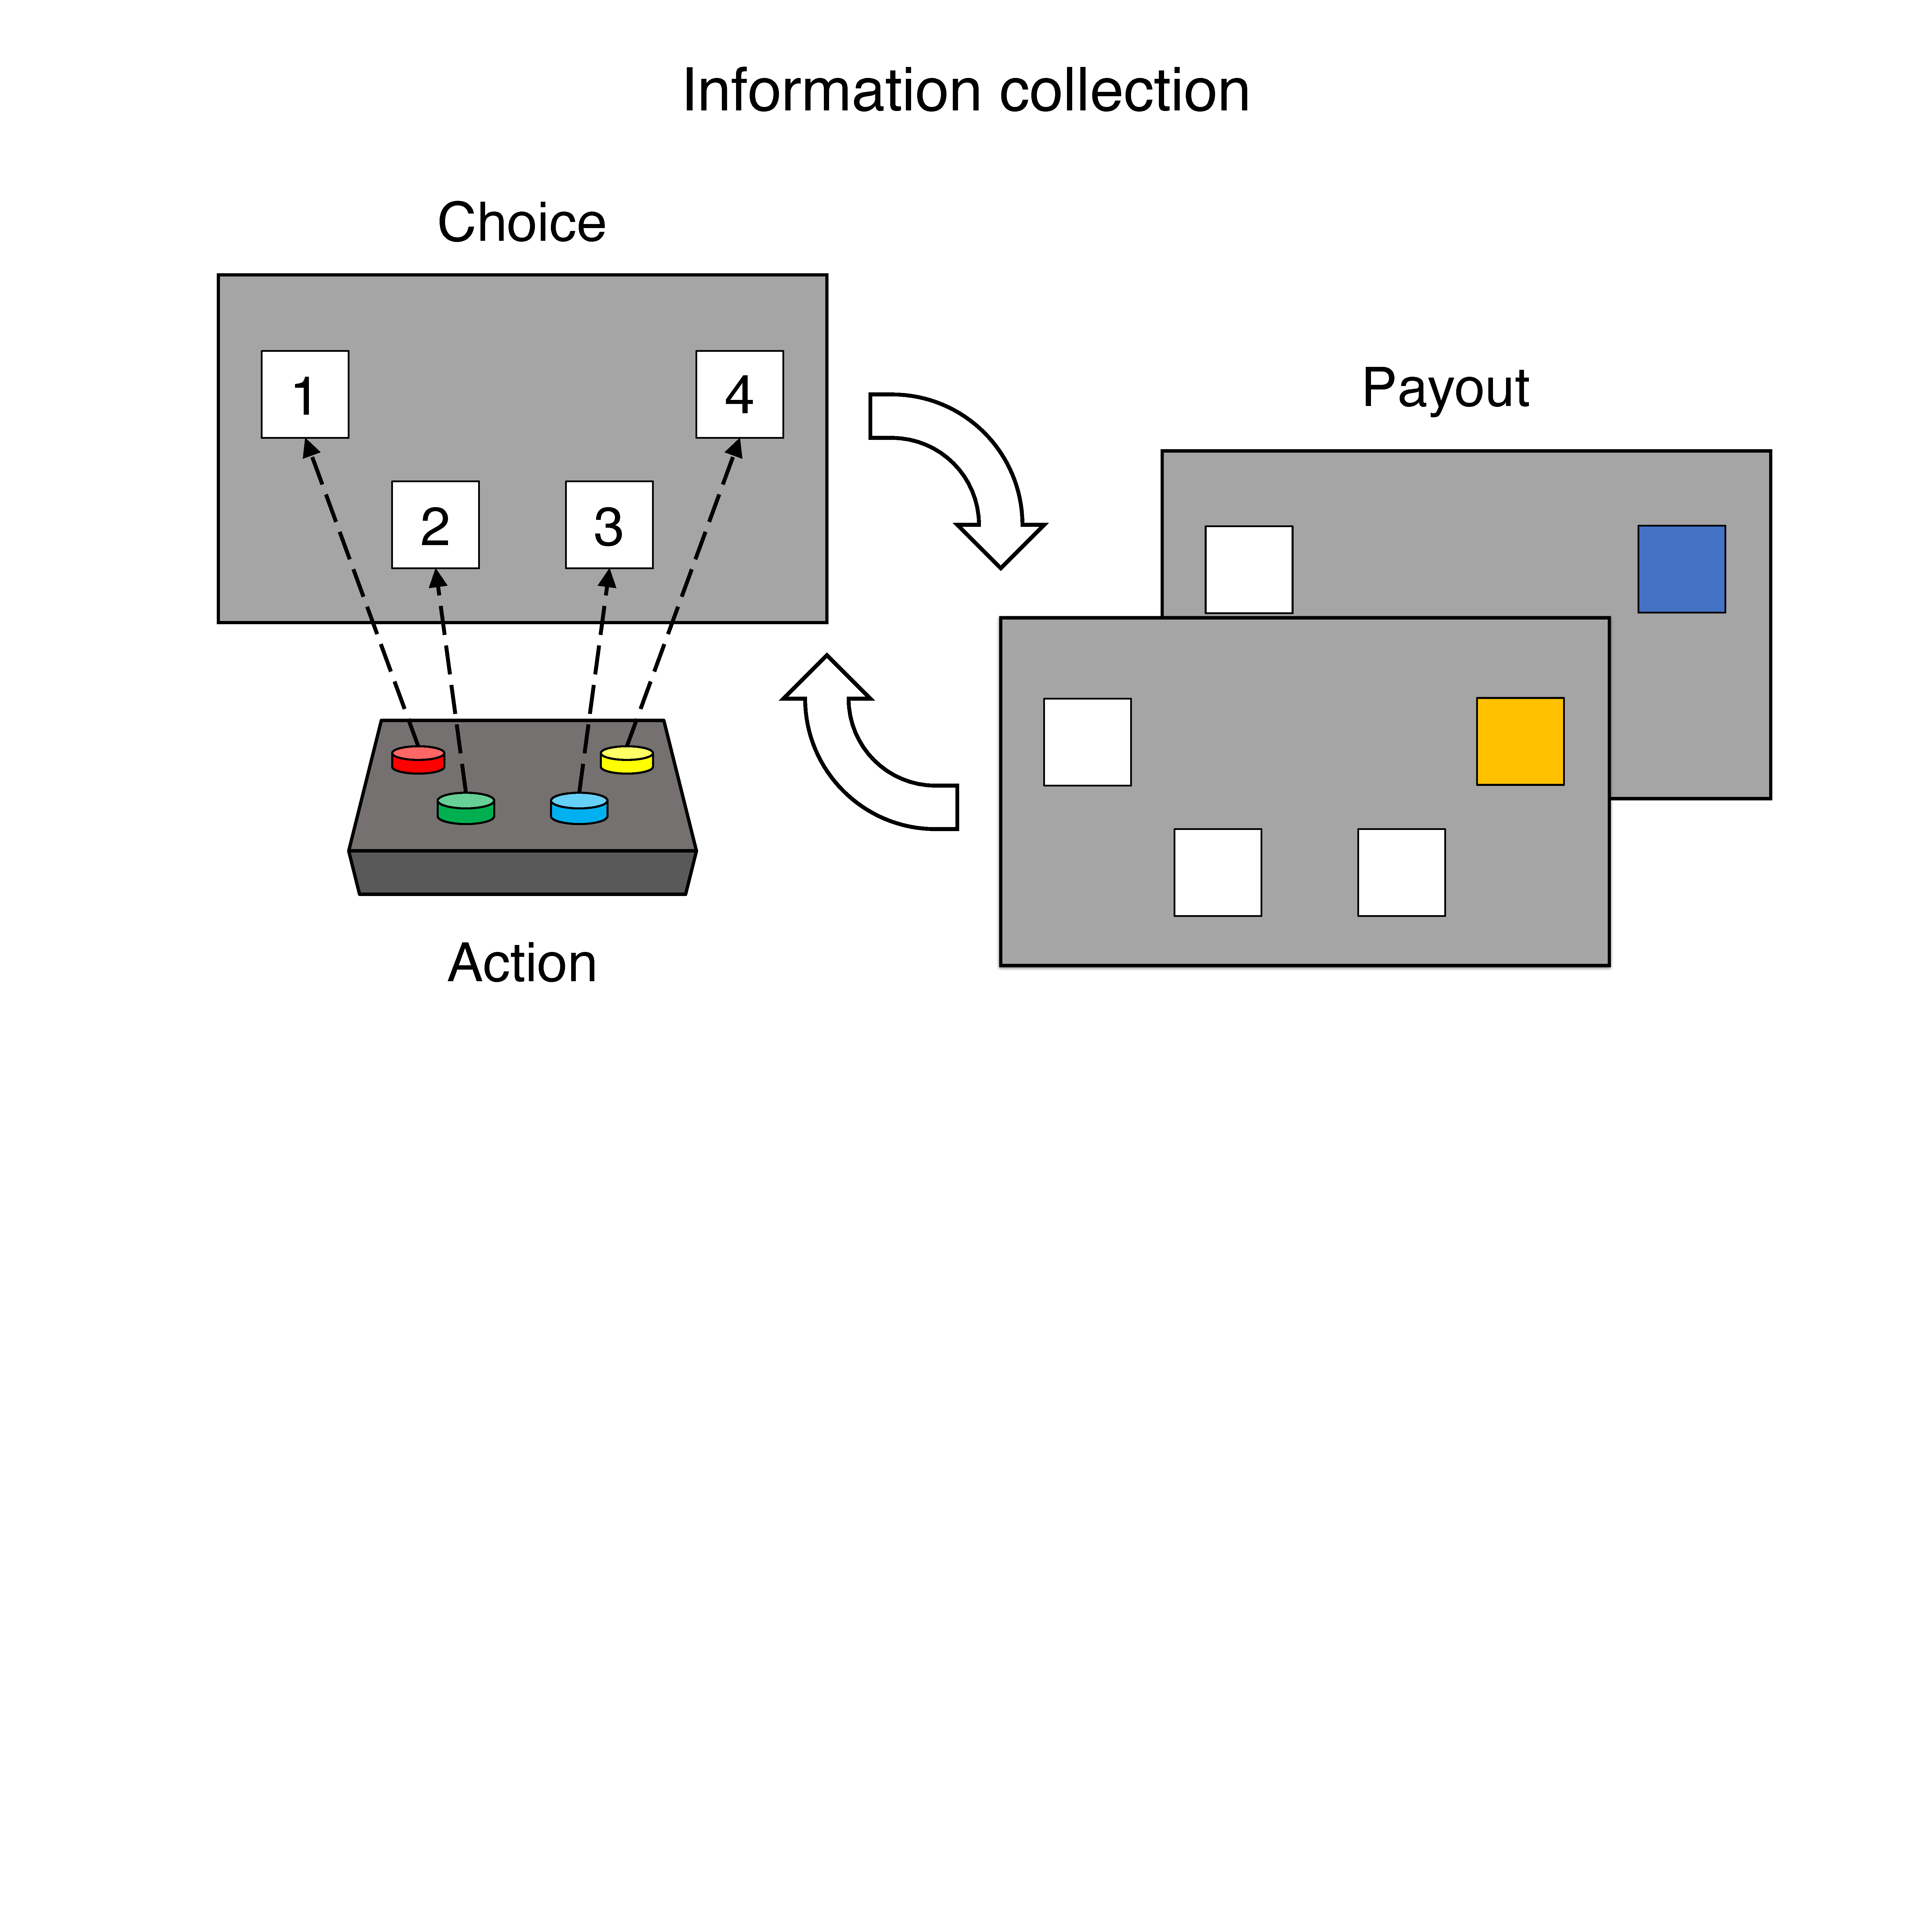
\includegraphics[width=0.7\linewidth]{img/task_outline1.pdf} 
	\caption{A simple four choice information foraging task. The information in this task is a yellow or blue stimulus, which can change from trial to trial. A good learner in this task is one who tries to learn the probabilities of all the symbols in each of the four choices. The more random the stimuli are in a choice, the more potential information/entropy there is to learn. \textit{Note}: the information payout structure is shown below (Fig.~\ref{fig:task_payout}a}).
	\label{fig:task_outline1} 
\end{figure}

\begin{figure}
	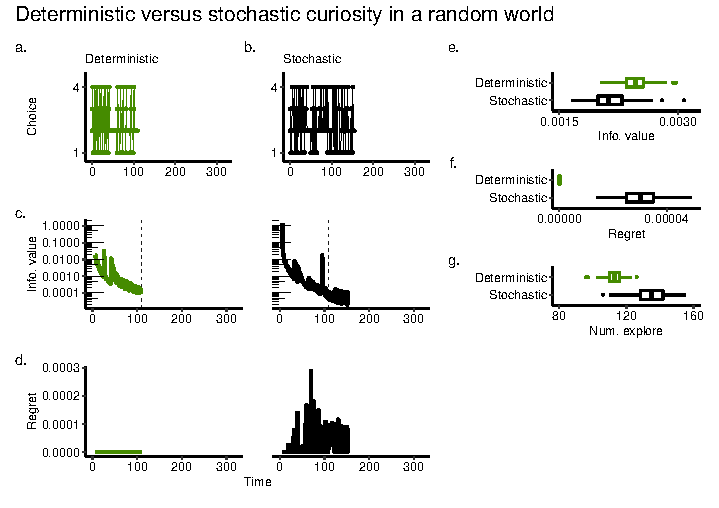
\includegraphics[width=1.0\linewidth]{img/curiosity1.pdf} 
	\caption{Comparing deterministic versus stochastic variations of the same curiosity algorithm, in a simple information foraging task (Task 1). Deterministic results are shown in the left column, and stochastic are shown in the right. The hyperparameters for both models were found by random search, which is described in the Methods.
	\textbf{a-b}. Examples of choice behavior.
	\textbf{c-d}. Information value plotted with time for the behavior shown in a-b.
	\textbf{e-f}. Regret plotted with time for the behavior shown in a-b. Note how our only deterministic curiosity generates zero regret, inline with theoretical predictions.
	\textbf{e}. Average information value for 100 independent simulations. Large values mean a more efficient search.
	\textbf{f}. Average regret for 100 independent simulations. Ideal exploration should have no regret. 
	\textbf{g}. Number of steps it took to reach the boredom threshold $eta$. Smaller values imply a faster search.
	}
	\label{fig:curiosity1} 
\end{figure}


\subsubsection*{Reward collection} 
We cannot mathematically ensure a mixed value solution to explore-exploit problems will maximizes reward value better than other well-established methods. To find out if this is so, we measured total reward collected over 7 tasks and 10 agents. Each agent's parameters were independently optimized for each task. For a brief description of each agent, see Table~\ref{tab:agents}. They all have in common that their central goal is to maximize total reward value, though this is often supplemented by some other goal, an intrinsic reward or bonus \cite{Ng1999,Sutton1998}. 

The general form of the 7 tasks are depicted in Fig~\ref{fig:task_outline2}. As with our first task (Fig. ~\ref{fig:task_outline1}) they are all variations of the classic multi-armed bandit \cite{Sutton2018}. The payouts for each of the tasks are shown separately in Fig.~\ref{fig:task_payout}. Every trial has a set of $n$ choices. Each choice returns a ``payout’’, according to a predetermined probability. Payouts are information, a reward, or both. Note that, as in Task 1, information was symbolic, denoted by a color code, ``yellow’’ and ``blue’’ and as is custom reward was a positive real number. 

The results in full for all tasks and exploration strategies are shown in Fig.~\ref{fig:summary}. All agents, including ours, used the same exploitation policy based on the temporal difference learning rule \cite{Sutton2018} (Methods).

\begin{figure}
	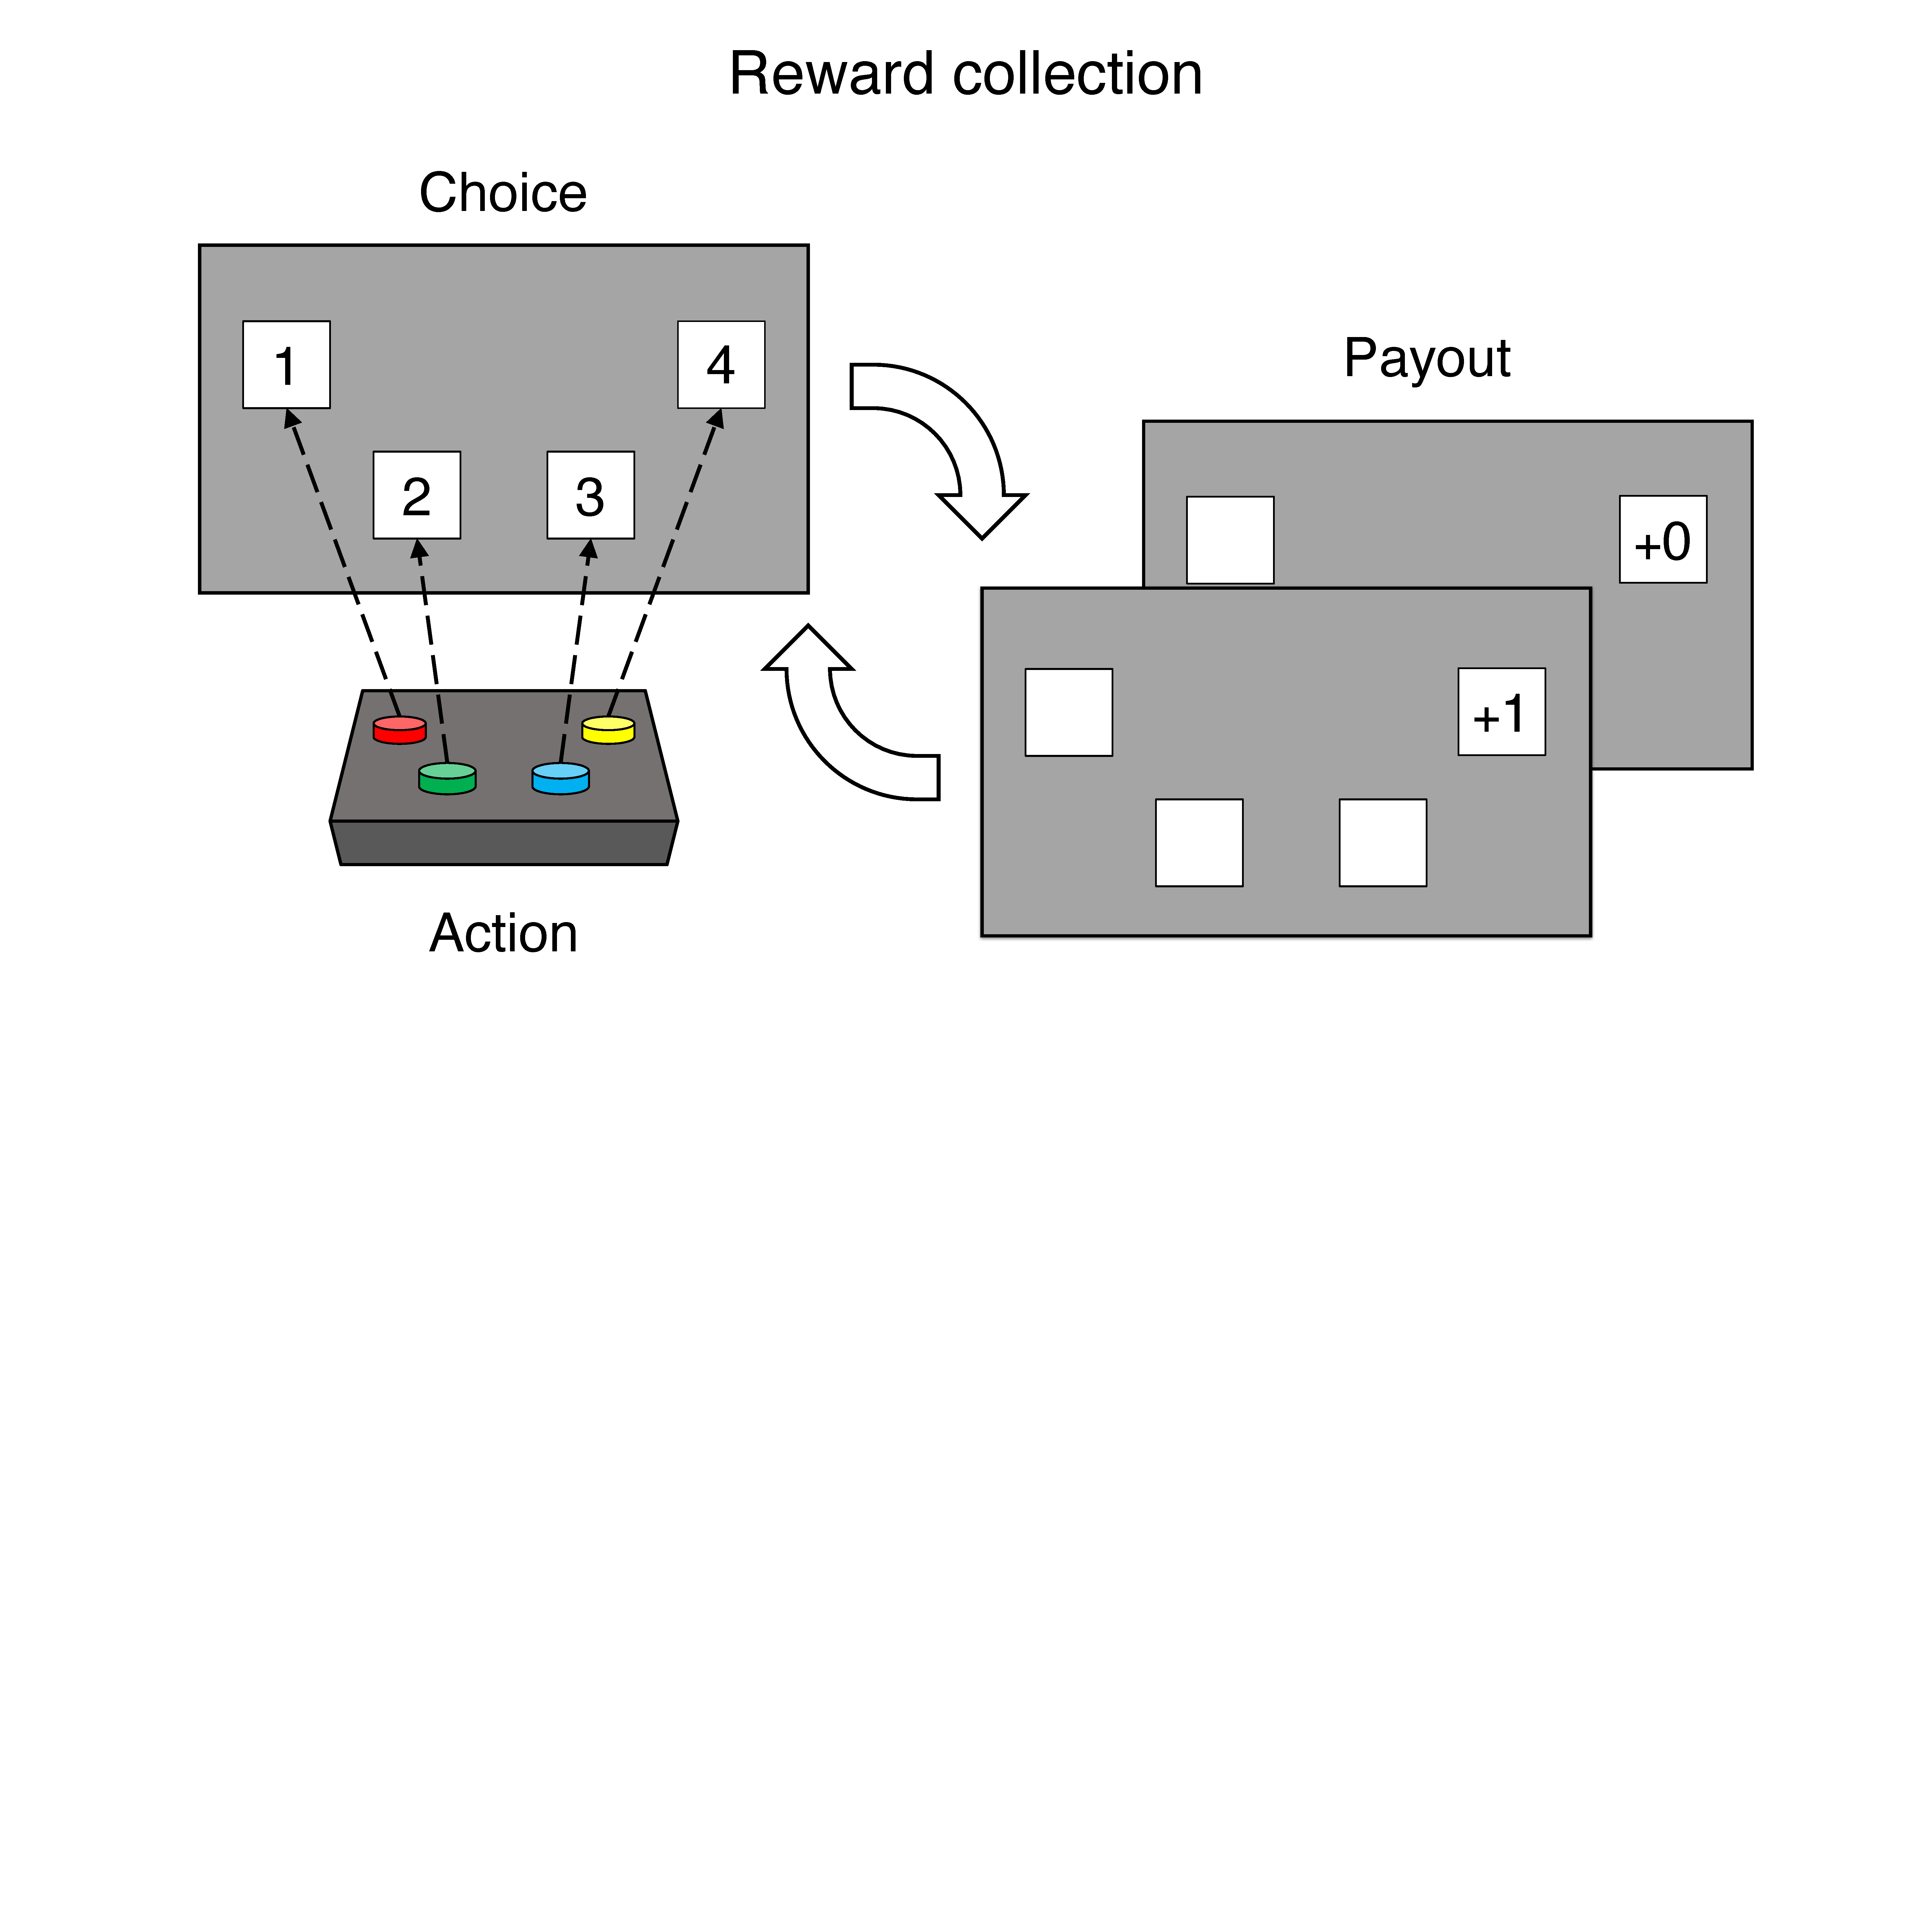
\includegraphics[width=0.7\linewidth]{img/task_outline2.pdf} 
	\caption{A 4 choice reward collection task. The reward is numerical value, here a 1 or 0. A good learner in this task is one who collects the most rewards. The task depicted here matches that in Fig~\ref{fig:task_payout}b. Every other reward collection task we study has the same basic form, only the number of choices increases and the reward spaces are more complex.}
	\label{fig:task_outline2} 
\end{figure}

\begin{SCfigure*}[\sidecaptionrelwidth][t]
    \label{fig:task_payout} 
	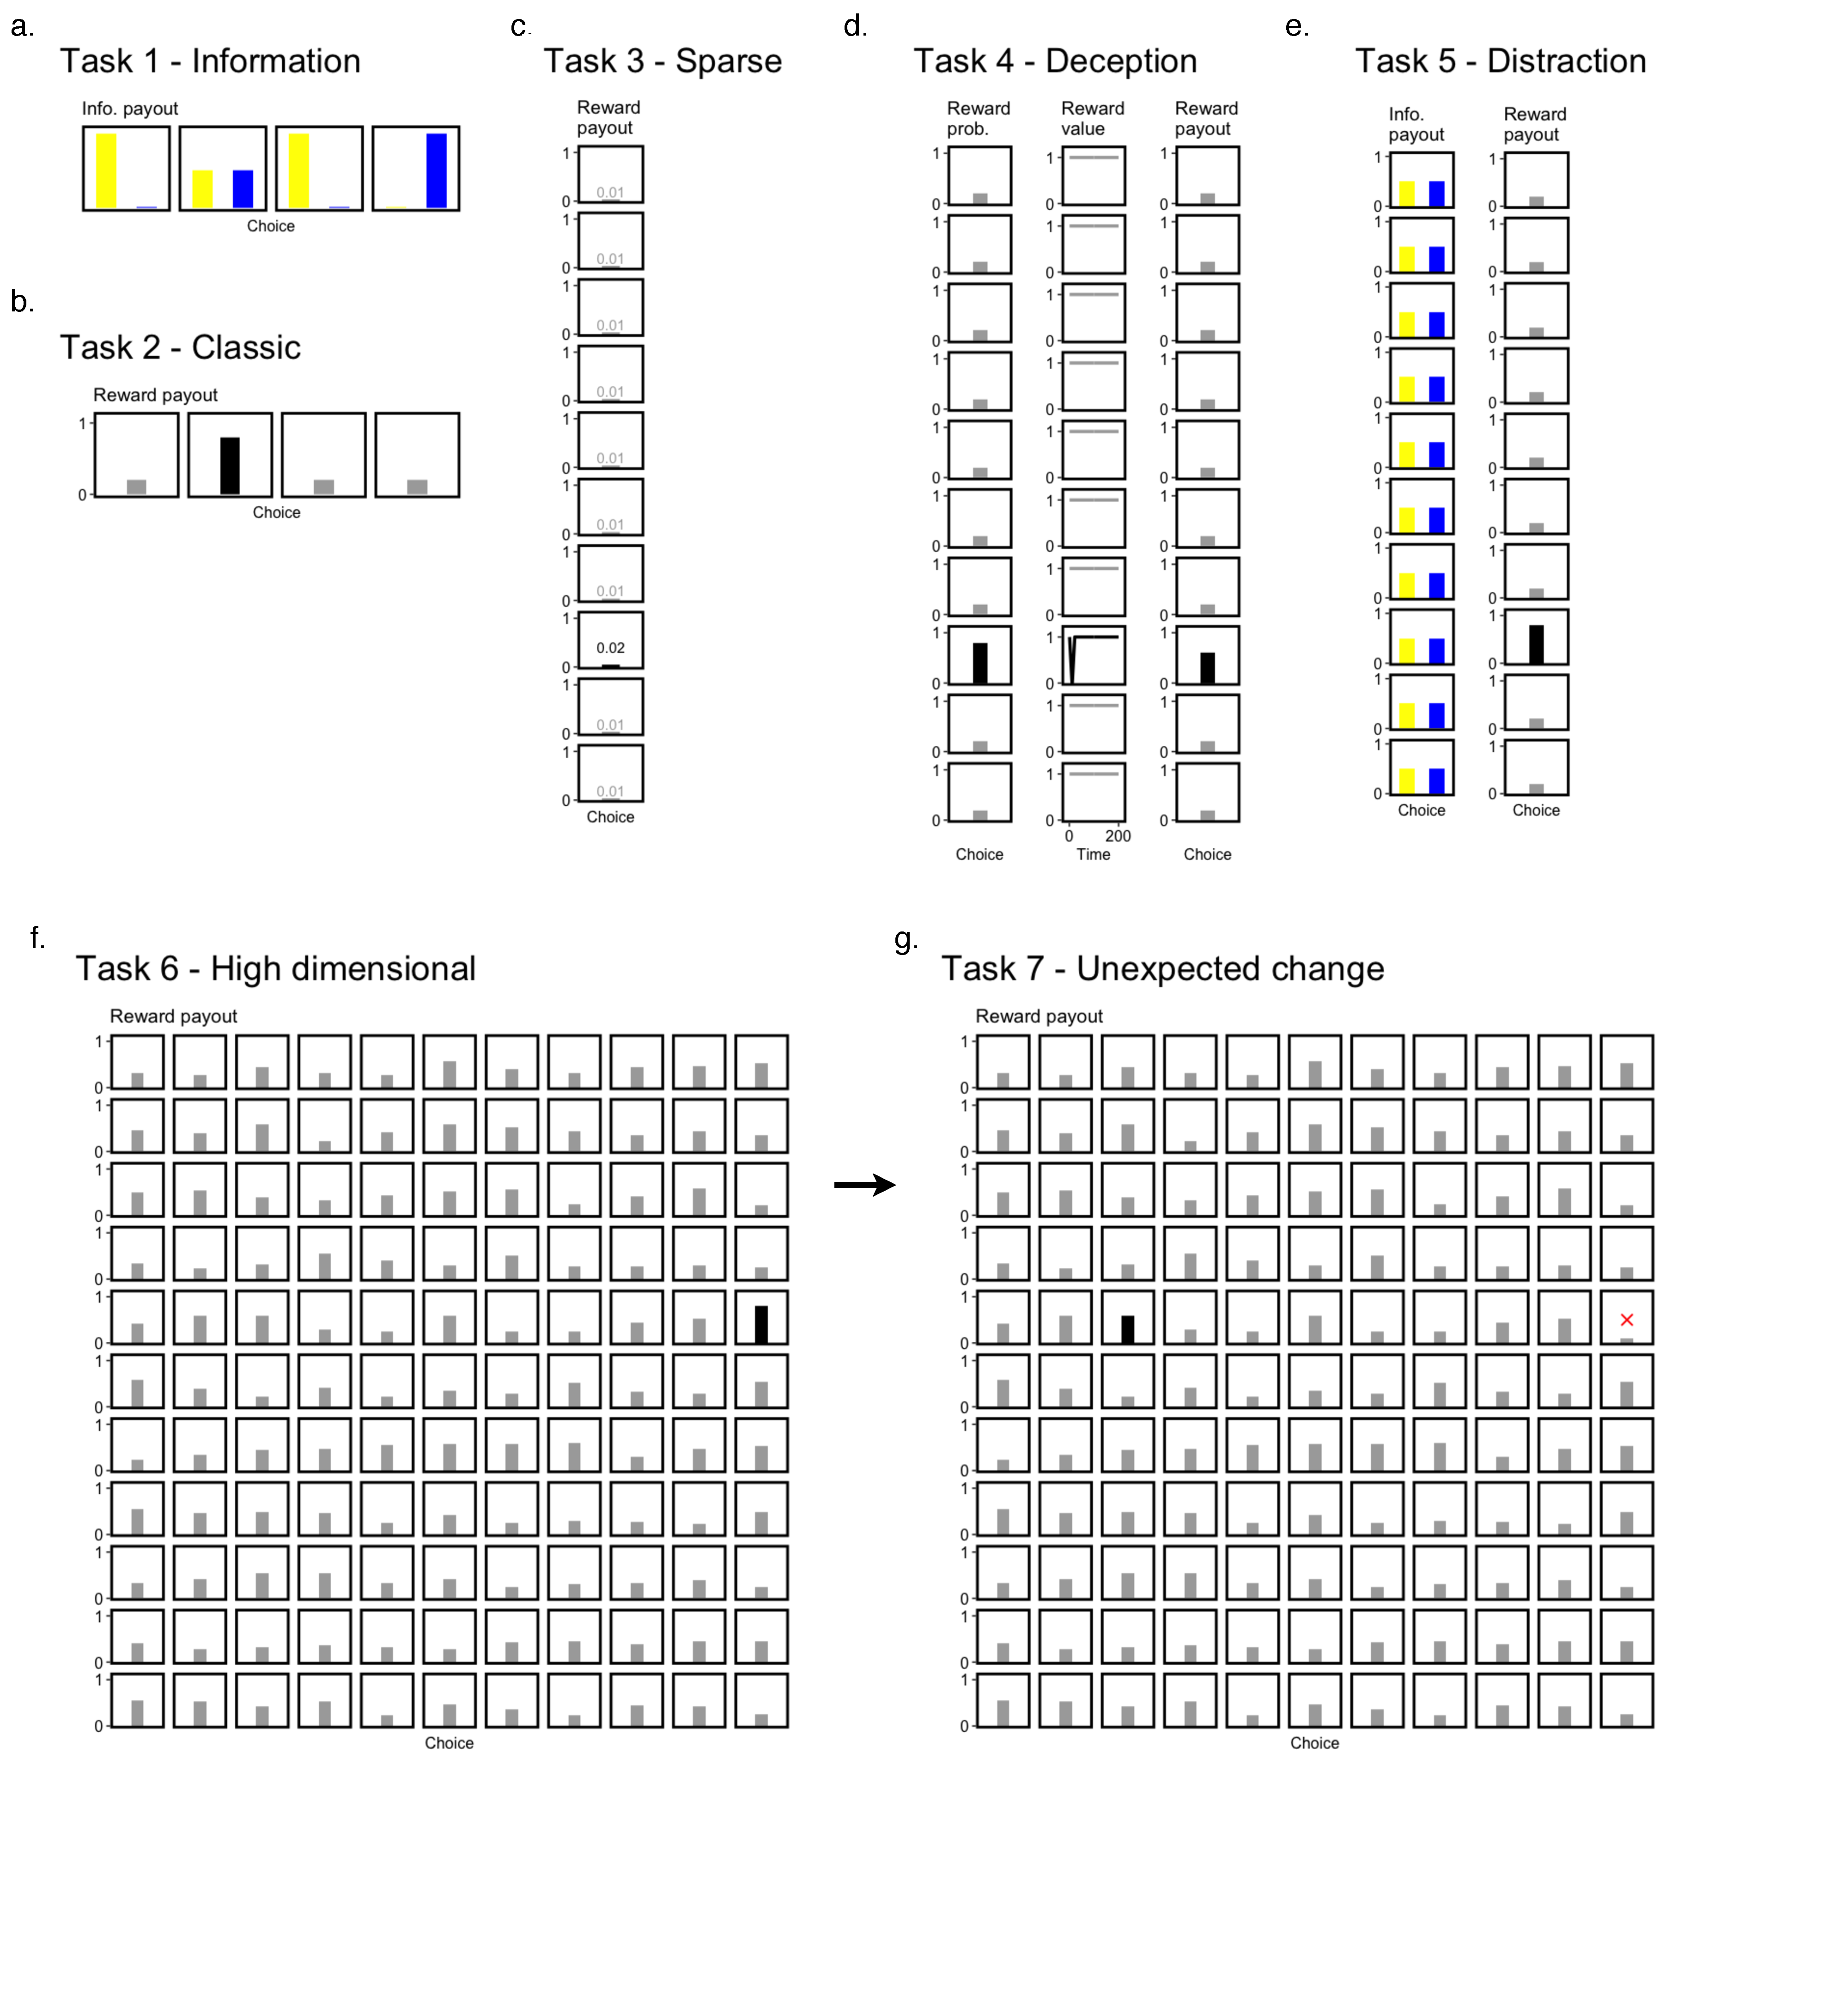
\includegraphics[width=11.4cm]{img/task_payout.pdf} 
	\caption{Payouts for \textit{Tasks 1 - 7}. Payouts can be information, reward, or both. For comments on general task design, see Fig~\ref{fig:task_outline2}.
	\textbf{a.} A classic four-choice design for information collection. A good learner should visit each arm, but quickly discover that only arm two is information bearing.
	\textbf{b.} A classic four-choice design for testing exploration under reward collection. The learner is presented with four choices and it must discover which choice yields the highest average reward. In this task that is Choice 2. 
	\textbf{c.} A ten choice sparse reward task. The learner is presented with four choices and it must discover which choice yields the highest average reward. In this task that is Choice 8 but the very low overall rate of rewards makes this difficult to discover. Solving this task with consistency means consistent exploration. 
	\textbf{d.} A ten choice deceptive reward task. The learner is presented with 10 choices, but the choice which is the best on the long-term (>30 trials) has a lower value in the short term. This value first declines, then rises (see column 2).
	\textbf{e.} A ten choice information distraction task. The learner is presented with both information and rewards. A good learner though will realize the information does not predict reward collection, and so will ignore it.
	\textbf{f.} A 121 choice task with a complex payout structure. This task is thought to be at the limit of human performance. A good learner will eventually discover choice number 57 has the highest payout.
	\textbf{g.} This task is identical to \textit{a.}, except for the high payout choice being changed to be the lowest possible payout. This task tests how well different exploration strategies adjust to simple but sudden change in the environment.
	}
	\label{fig:task_payout} 
\end{SCfigure*}

\begin{table}[]
	\caption{Exploration strategies.}
	\label{tab:agents}
	\begin{tabular}{|p{2cm}|p{2cm}|p{3cm}|}
	\hline
	\textbf{Name} & \textbf{Class} & \textbf{Exploration strategy} \\ \hline
	Curiosity & Deterministic & Maximize information value \\ \hline
	Random/Greedy & Random & Alternates between random exploration and greedy with probability $\epsilon$. \\ \hline
	Decay/Greedy & Random & The $\epsilon$ parameter decays with a half-life \\ \hline
	Random & Random & Pure random exploration \\ \hline
	Reward & Directed & Softmax sampling of reward value \\ \hline
	Bayesian & Directed & Softmax sampling of reward value + information value \\ \hline
	Novelty & Directed & Softmax sampling of reward value + novelty signal \\ \hline
	Entropy & Directed & Softmax sampling of reward value + action entropy \\ \hline
	Count (EB) & Directed & Softmax sampling of reward value + visit counts \\ \hline
	Count (UCB) & Directed & Softmax sampling of reward value + visit counts \\ \hline
	\end{tabular}
\end{table}

\begin{SCfigure*}[\sidecaptionrelwidth][t]
	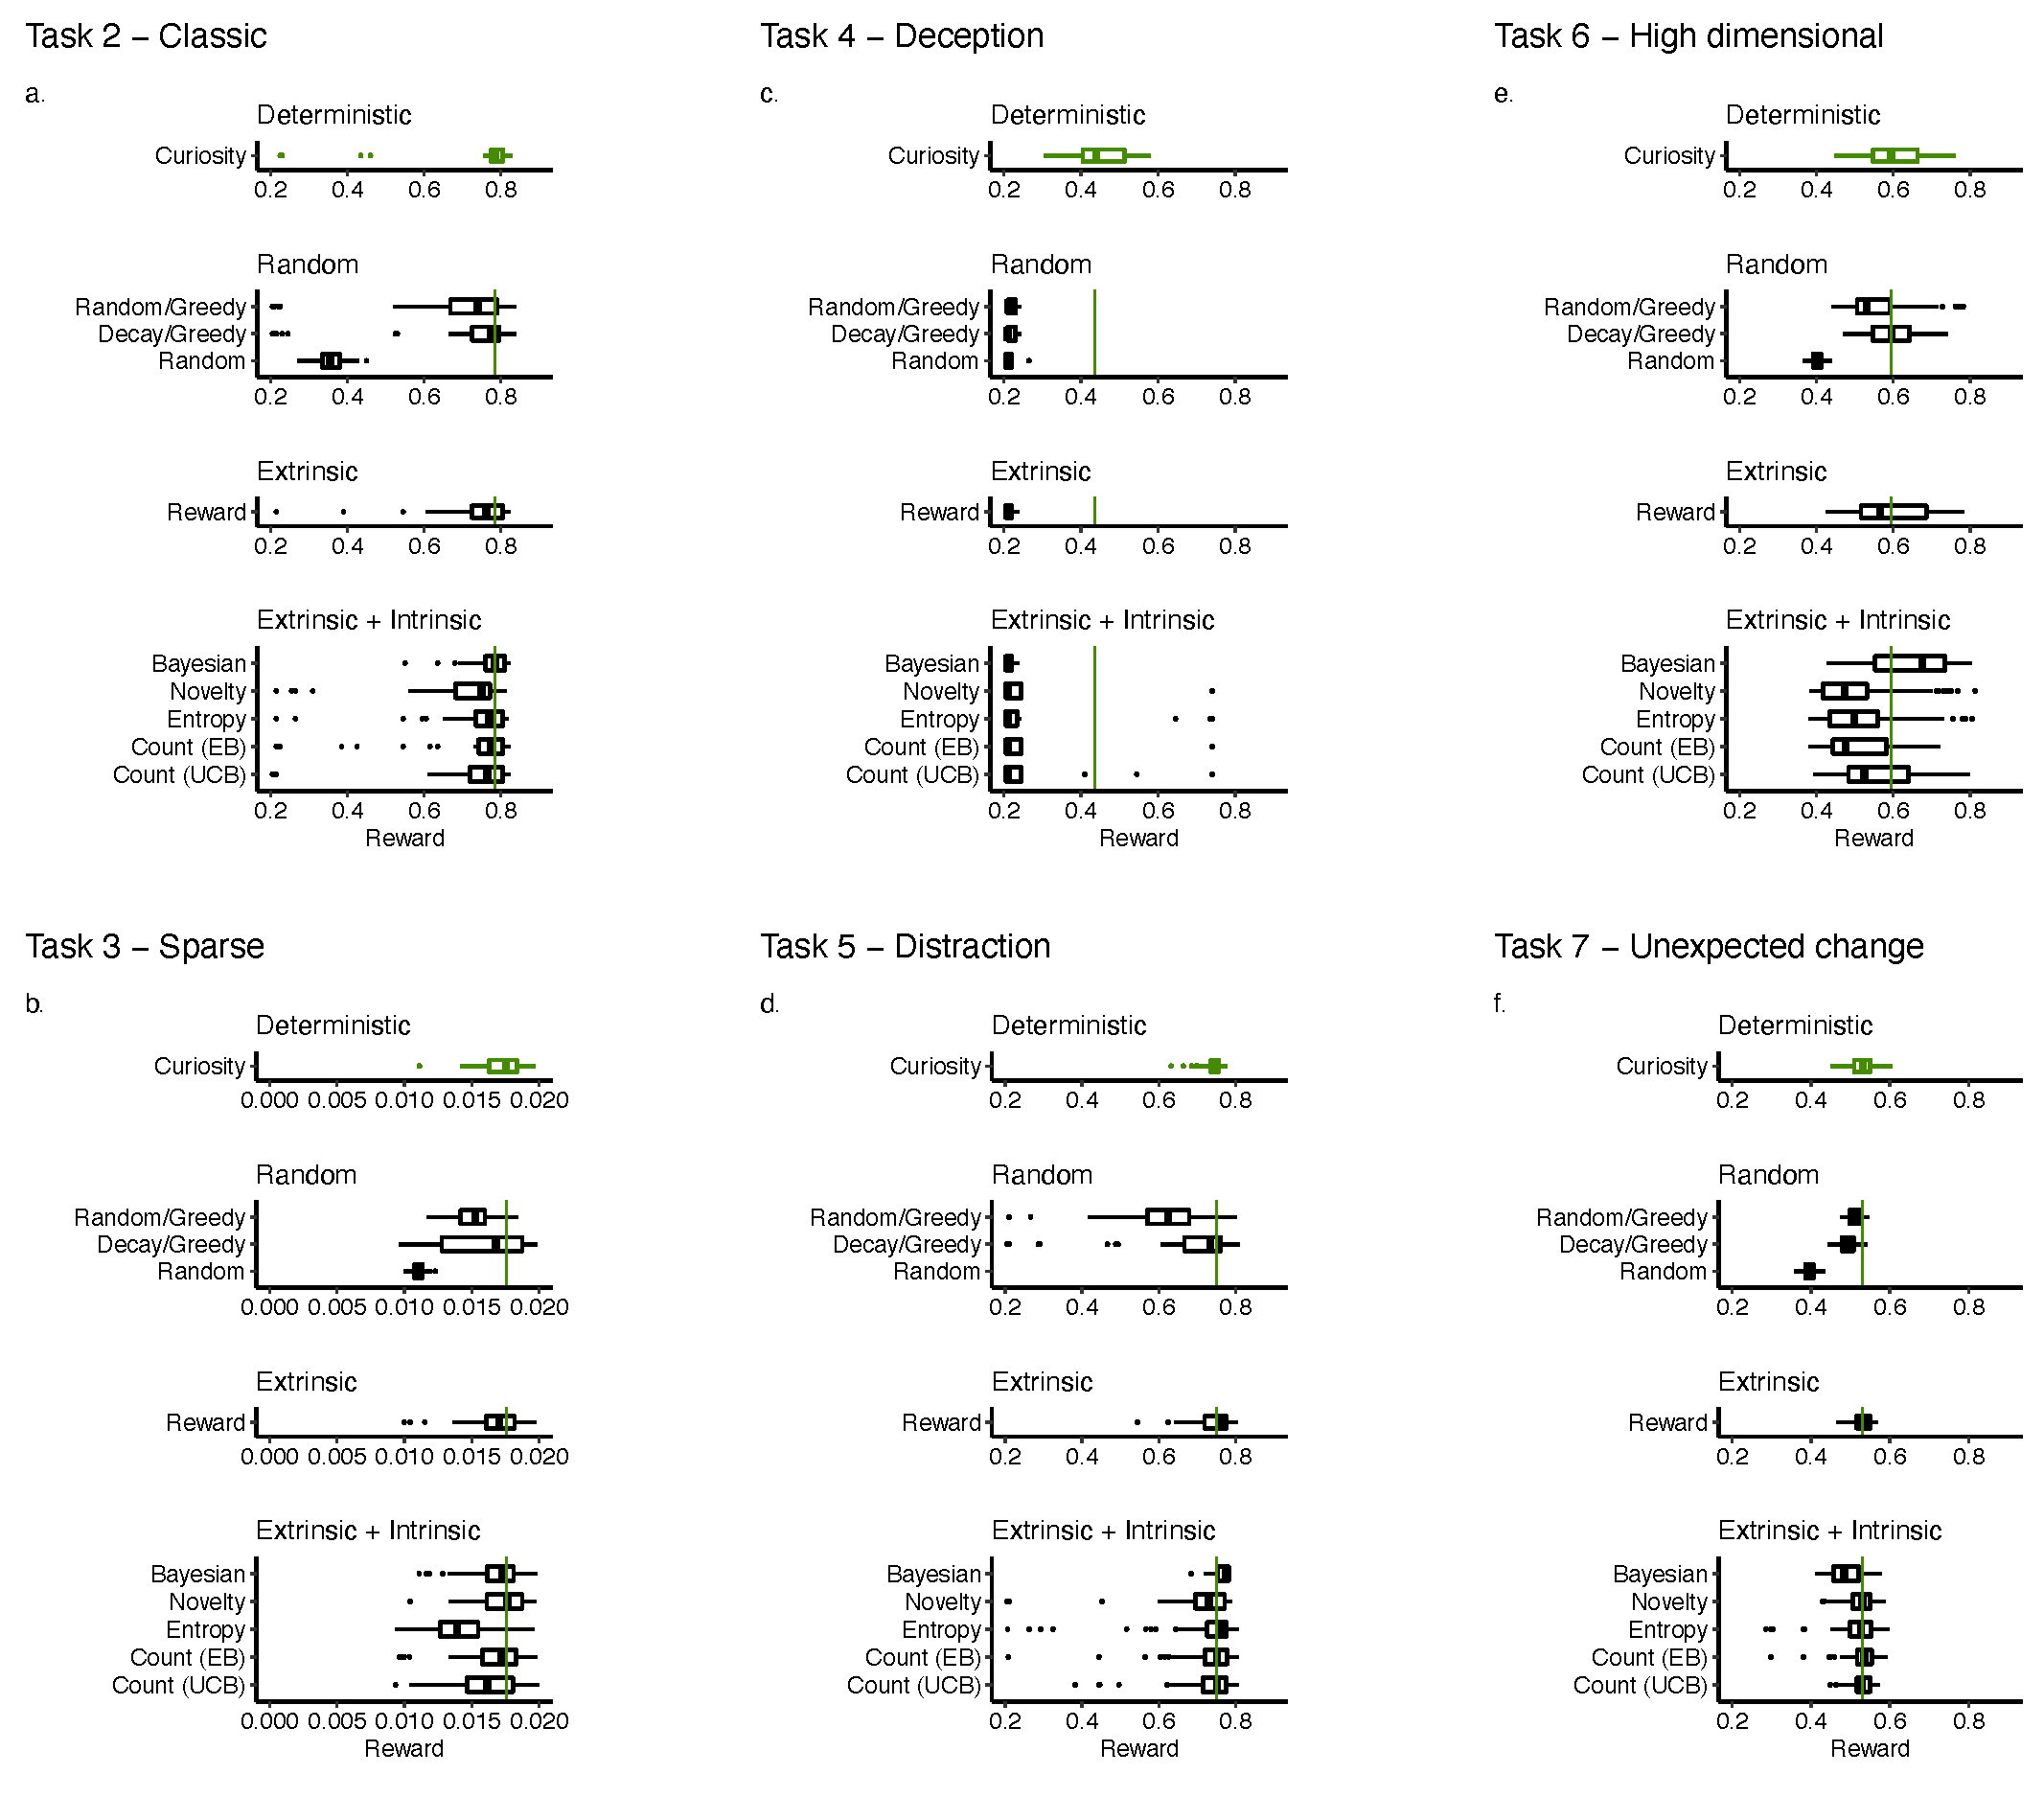
\includegraphics[width=11.4cm]{img/summary.pdf} 
	\caption{Summary of reward collection (\textit{Tasks 2-7}). The strategies in each panel are grouped according to the class of search they employed (Curiosity. Random, Extrinsic reward or Extrinsic + Intrinsic rewards). 
	\textbf{a.} Results for Task 2, which has four choices and one clear best choice.
	\textbf{b.} Results for Task 3, which has 10 choices and very sparse positive returns.
	\textbf{c.} Results for Task 4, whose best choice is initially ``deceptive'' in that it returns suboptimal reward value over the first 20 trials.
	\textbf{d.} Results for Task 5, which blends the information foraging task 1 with a larger version of Task 2. The yellow/blue stimuli are a max entropy distraction which do not predict the reward payout of each arm.
	\textbf{e.} Results for Task 6, which has 121 choices and a quite heterogeneous set of payouts but still with one best choice.
	\textbf{f.} Results for Task 7, which is identical to Task 6 except the best choice was changed to be the worst. The learners from Task 6 were trained on this Task beginning with the learned values from their prior experience -- a test of robustness to sudden change in the environment. 
	\textit{Note}: To accommodate the fact that different tasks were run different numbers of trials, we normalized total reward by trial number. This lets us plot reward collection results for all tasks on the same scale.
  	}	
	\label{fig:summary} 
\end{SCfigure*}

\begin{SCfigure*}[\sidecaptionrelwidth][t]
    \label{fig:supp_regret} 
	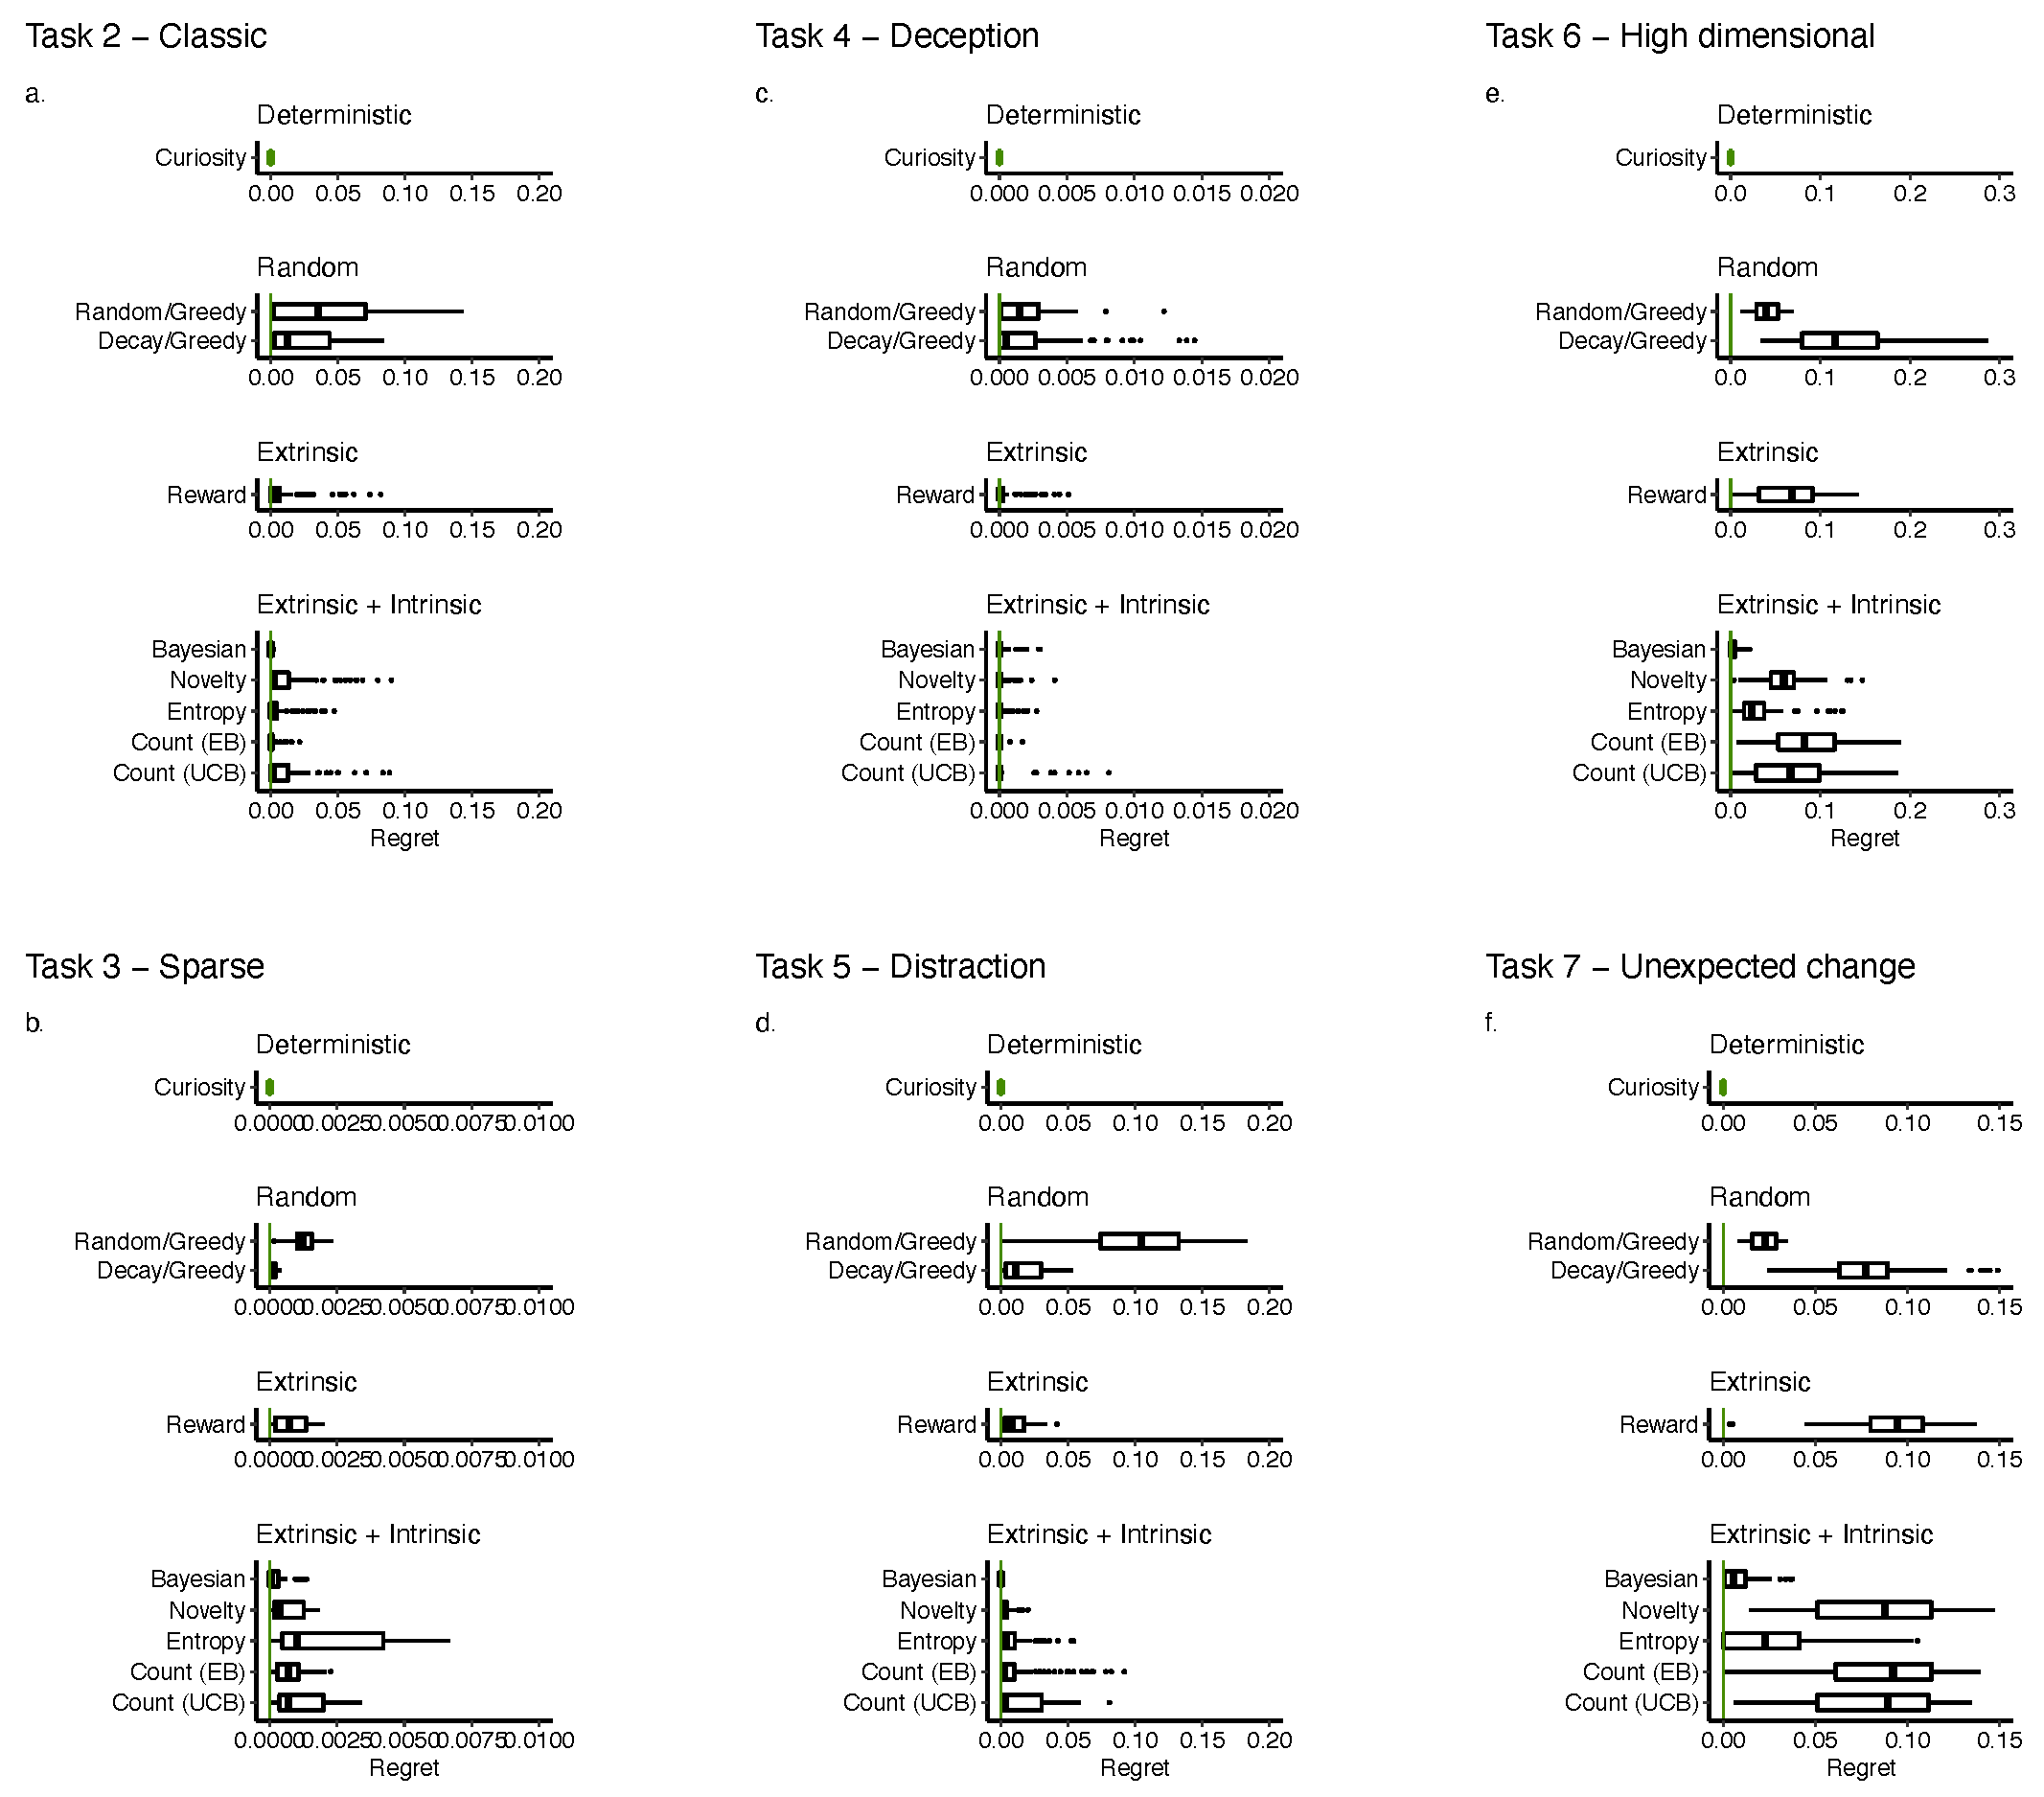
\includegraphics[width=11.4cm]{img/supp_regret.pdf} 
	\caption{Summary of total regret (\textit{Tasks 2-7}). See the previous figure for details.}
\end{SCfigure*}

% \begin{SCfigure*}[\sidecaptionrelwidth][t]
%     \label{fig:exploration1} 
% 	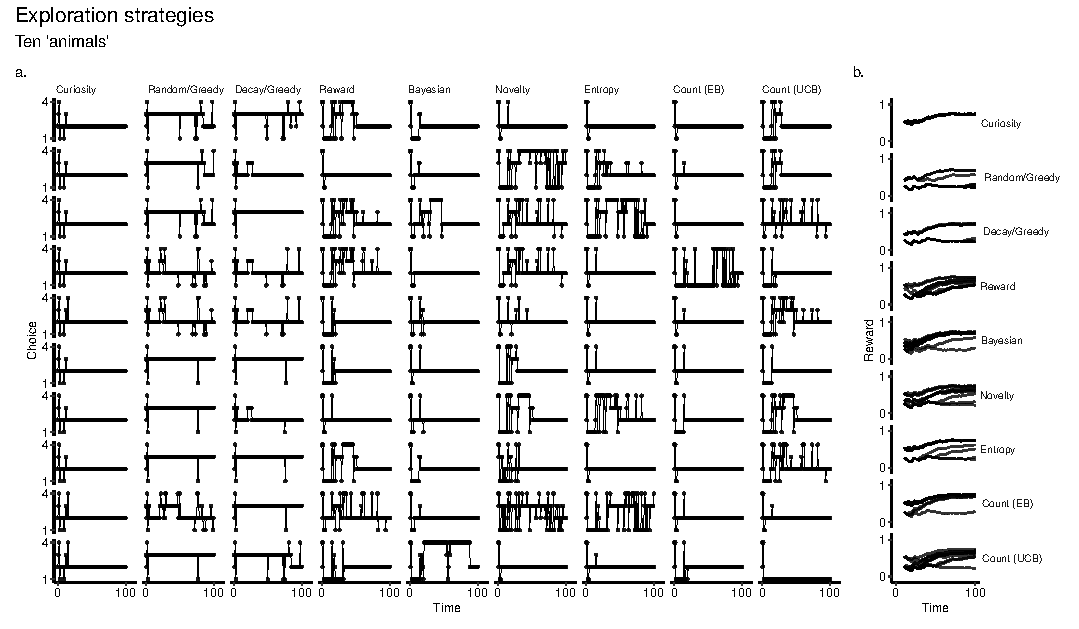
\includegraphics[width=11.4cm]{img/exploration1.pdf}
% 	\caption{Variance in exploration strategies for 10 ``animals'' (Task 1). Here we simulated a single random seed, on the same task. Model parameters were the top-10, for each strategy. In this Figure we consider each of these parameters to act as a stand in for a unique ``animal''. This figure then estimates the degree, and kind, of variability expected which would be expected in the same experiment for different (well-adapted) animals. Note the reduced variability seen when using curiosity, compared to the others.
%   	}
% \end{SCfigure*}

\textit{Task 1} is an information gathering task, which we discussed above.  We present the design and results here to contrast with the reward collection tasks. 

\textit{Task 2} was designed to examine reward collection, in probabilistic reward setting very common in the decision making literature \cite{schonberg2007reinforcement,frank2004carrot,cavanagh2014conflict,jahfari2019cross,collins2014opponent,collins2017interactions,glascher2010states}. Rewards were 0 or 1. The best choice had a payout of $p(R=1) = 0.8$. This is a much higher average payout than the others ($p(R=1) = 0.2$). At no point does the task generate symbolic information. See, Fig.~\ref{fig:task_payout}\textbf{b}. 

In contrast to the performance in Task 1, in Task 2 we expected all the exploration strategies to succeed. While this was indeed the case, our deterministic curiosity was the top-performer in terms of median rewards collected, though by a small margin (Fig.~\ref{fig:summary}\textbf{a}).

\textit{Task 3} was designed with very sparse rewards \cite{Silver2016b,Silver2018} and there were 10 choices, making this a more difficult task (Fig.~\ref{fig:task_payout}\textbf{c}). Sparse rewards are a common problem in the natural world, where an animal may have to travel and search between each meal This is a difficult but not impossible task for vertebrates \cite{anderson1984optimal} and invertebrates \cite{westphal2006foraging}. That being said, most reinforcement learning algorithms will struggle in this setting because the thing they need to learn, that is rewards, are often absent. In this task we saw quite a bit more variation in performance, with the novelty-bonus strategy taking the top slot (this is the only time it does so).

\textit{Task 4} was designed with deceptive rewards. By deceptive we mean that the best long-term option presents itself initially with a decreasing reward value (Fig.~\ref{fig:task_payout}\textbf{d}). Such small deceptions abound in many natural contexts where one must often make short-term sacrifices \cite{internicola2012bumble}. It is well known that classic reinforcement learning will often struggle in this kind of task \cite{Lehman2011a,Sutton2018}. Here our deterministic curiosity is the only strategy that reaches above chance performance. Median performance of all other strategies are similar to the random control (Fig~\ref{fig:summary}\textbf{c}). 

\textit{Task 5} was designed to fool curiosity, our algorithm, by presenting information that was utterly irrelevant to reward collection, but had very high entropy and so ``interesting'' to our algorithm. We fully anticipated that this context would fool just our algorithm, with all other strategies performing well since they are largely agnostic to entropy. However, despite being designed to fail, deterministic curiosity still produced a competitive performance to the other strategies (Fig~\ref{fig:summary}\textbf{d}). 

\textit{Tasks 6-7} were designed as a pair, with both having 121 choices, and a complex payout structure. Tasks of this size are at the limit of human performance \cite{Wu2018}. We first trained all learners on \textit{Task 6}, then tested them in Task 7 which identical to 6, except the best payout arm is reset to be worst (Fig.~\ref{fig:task_payout}\textbf{e}-\textbf{f}). In other words Tasks 6 and 7 were joined to measure learning in a high dimensional, but shifting, environments.

In Task 6 deterministic curiosity performed well, securing a second place finish. We note the Bayesian strategy  outperformed our approach. However, under the sudden non-stationarity in reward when switching tasks, the top Bayesian model became the worst on Task 7, and deterministic curiosity took the top spot. Compare Fig.~\ref{fig:summary}\textbf{e} to \textbf{f}. This is the robustness that we'd expect for any curiosity algorithm, whose main goal is to learn everything unbiased by other objectives. The environment and the objectives do change in real life, and so we must be prepared for this. Note how the other less-biased-toward-reward-value exploration models (count-based, novelty, and entropy models) also saw gains, to a lesser degree.

\subsubsection*{Robustness}
It is common to focus on best case performance, as we have above. However worst case performance is just as important in judging the usefulness of an algorithm. We therefore examined the progression from best case hyperparameters, to the worst case.  

Unlike idealized simulations, animals cannot know with perfect fidelity how their environment may change. So they cannot perfectly know the search parameters, in other words. To test the robustness of our algorithm, and all other exploration strategies we considered, we reexamined reward collection performance across all hyperparameters from our tuning set. Results for this are shown in Figure~\ref{fig:robust}. We plotted performance ranked by parameters, from best to worst.

\begin{SCfigure*}[\sidecaptionrelwidth][t]
	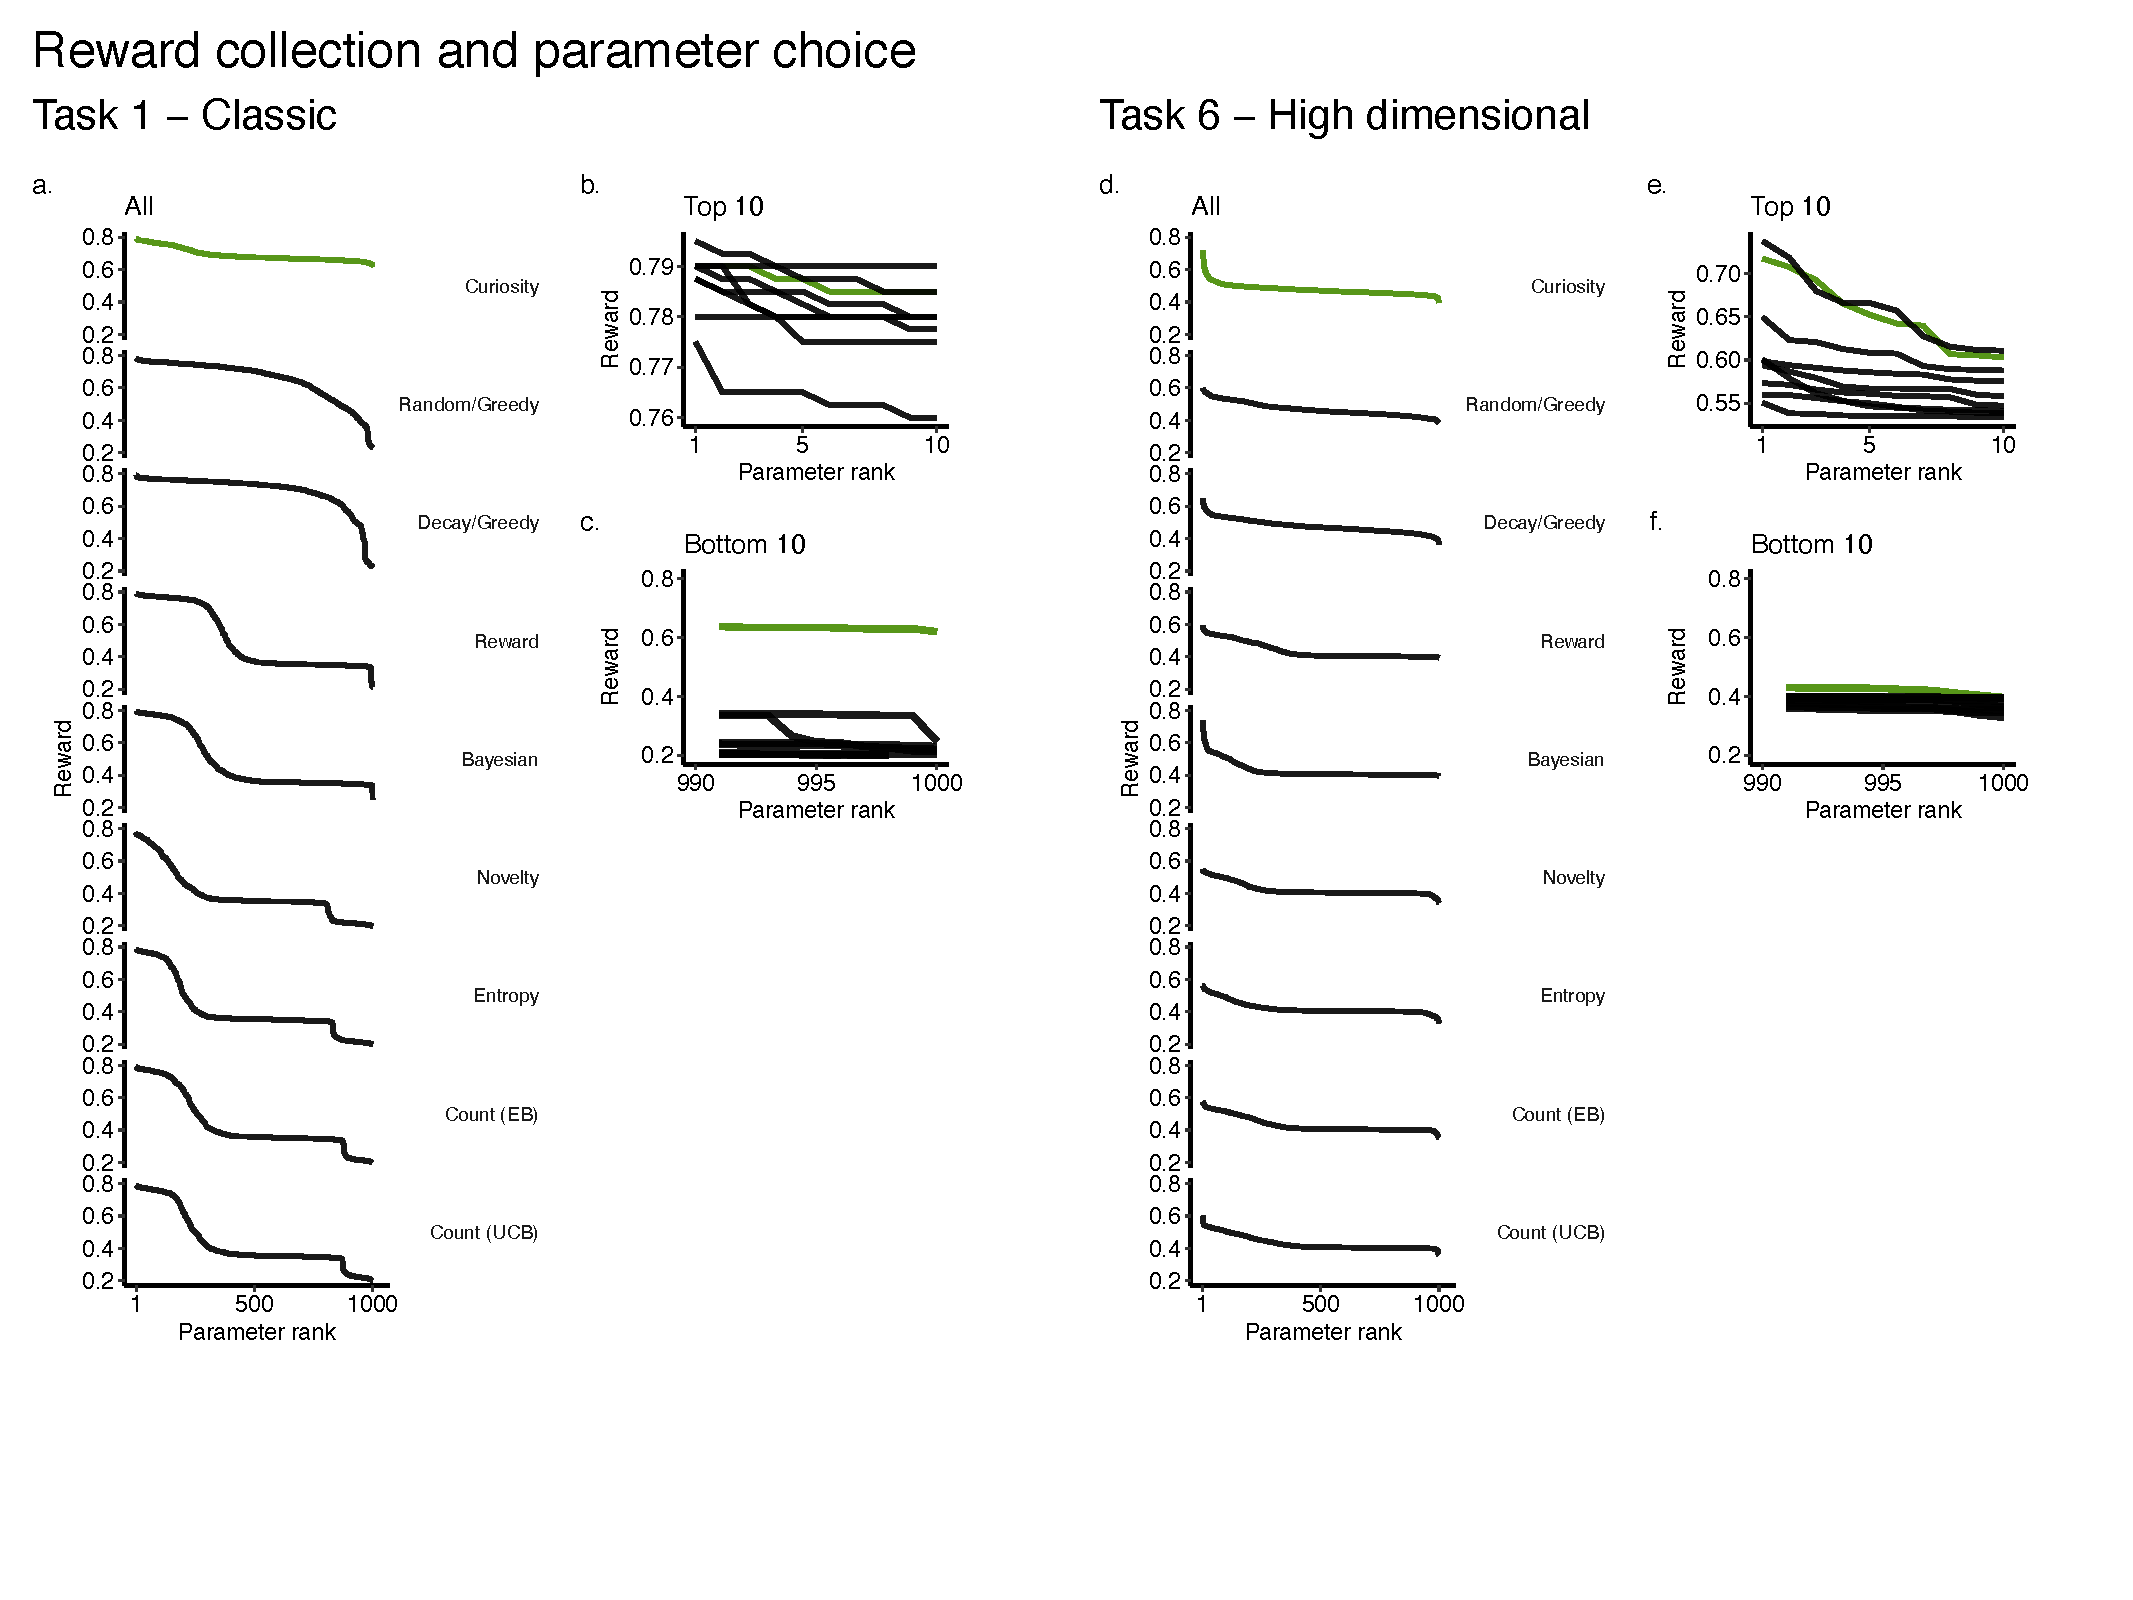
\includegraphics[width=11.4cm]{img/robust.pdf} 
	\caption{Parameter sensitivity (\textit{Task 2} and \textit{6}). Here we evaluated how robust performance was for random hyperparameters, rather than those which were carefully chosen. A very robustness exploration algorithm would produce strong performance with both the best parameter choices, and the worst parameter choices. 
	\textbf{a,d} Total reward for 1000 randomly choosed hyperparameters, for each of the agents.
	\textbf{b,e} Performance with the top 10 random hyperparameters, after ranking. Curiosity (green) compared to all the others.
	\textbf{c.f} Performance with the bottom 10 random hyperparameters, after ranking.
	}
	\label{fig:robust}
\end{SCfigure*}

No matter the parameter choices, exploration-as-curiosity produced top-3 performance (Figure.~\ref{fig:robust}a-bd). Most interesting to note is the performance on the worst 10 parameters. Here curiosity was markedly better, with substantially less variability.

All other exploration strategies we considered have hyperparameters to tune their \emph{degree} of exploration. For example, the temperature of noise in softmax. With our approach to curiosity, however, we tune only when exploration should stop, by $\eta$. In these examples, performance is more robust to  ``mistuning'' the stopping point, rather than the degree of exploration.

\section{Discussion}
We have offered a way around the dilemma where curiosity is how animals explore, in all circumstances. This is a controversial claim. So we'll address some of its criticisms, as a series of questions.


\subsection*{Is this too complex?}
Perhaps turning a single objective into two, as we have, is an unneeded complication. If this is true this it would mean ours is not a parsimonious solution to the dilemma, and so we could or should reject it on that alone. 

Questions about parsimony are resolved by considering the benefits versus the costs. The benefits to curiosity-based search is that it leads to no regret solutions to exploration, to exploration-exploitation, and that it so far seems to do very well in practice, at reward collection. At the sametime curiosity-as-exploration can also be building a model of the environment, useful for later planning \cite{Ahilan2019,Poucet1993}, creativity, imagination \cite{Schmidhuber2010}, while also building in some cases diverse action strategies \cite{Lehman2011a,Lehman2013,Mouret2015,Colas2020}. In other words, we argue it is a needed complication. 


\subsection*{Is this too simple?}
Solutions to the regular dilemma are complex and require sophisticated mathematical efforts and complex computations when compared to our solution. Or put another way, our solution may seem too simple. So have we ``cheated'' by changing the problem as we have?

The truth is we might be cheating in this sense. The dilemma might have to be as hard as it has seemed in the past. But the general case for curiosity as useful is clear, and backed up by the brute fact of its widespread presence in animals. The question is: is curiosity so useful and so robust that it can be sufficient for all exploration (with learning). 

The answer to this question is empirical. If our account does well in describing and predicting animal behavior, that would be some evidence for it. If it predicts neural structures \cite{Cisek2019}, that would be some evidence for it. If this theory proves useful in machine learning and artificial intelligence research, that would be some evidence for it.


\subsection*{Is this a slight of hand, theoretically?}
Yes. It is often useful in mathematical studies to take one problem that cannot be solved, and replace it with another related problem that can be. This is what we have done for exploration and the dilemma. The regular view of the problem has no tractable solution, without regret. Ours has a solution.


\subsection*{But isn't curiosity impractical?}
It does seem curiosity is just as likely to lead away from a needed solution, as towards it. Especially so if one watches children who are the prototypical curious explorers \cite{Sumner2019,Kidd2015}. This is why we limit curiosity with boredom, and counter it with a competing drive for reward collecting / exploitation. 

We believe there is a useful analogy between science and engineering. Science can be considered an open-ended inquiry, and engineering a purpose driven enterprise. They each have their own pursuits but they also learn from each other, often in alternating iterations \cite{Gupta2006}. It is their different objectives though which make them such good long-term collaborators.


\subsection*{But what about curiosity on big problems?}
A significant drawback to curiosity, as an algorithm, is that it will struggle to deliver timely results when the problem is very large, or highly detailed. First, it's worth noting that most learning algorithms struggle with this setting \cite{MacKay2003,Sutton2018}, unless that is unless significant prior knowledge can be brought to bear \cite{Zhang2020,Sutton2018} or the problem can be itself compressed \cite{Ha2018a,Fister2019}. Because however ``size'' is a widespread problem in learning, there are a number of possible solutions. And because our definition of learning, memory and curiosity is so general, we can take advantage of most. This does not guarantee curiosity will work out for all problems; all learning algorithms have counterexamples afterall \cite{Wolpert1997}.


\subsection*{But what about...?}
We did not intend to dismiss the niceties of curiosity, which others have revealed. It is that these prior divisions parcel out the idea too soon. Philosophy and psychology consider whether curiosity is internal or external, perceptual versus epistemic, or specific versus diversive, or kinesthetic \cite{Kidd2015,Berlyne1950,Zhou2020}. Computer science tends to define it as needed, for the task at hand \cite{Stanley2004,Friston2016,Lehman2011a,Lehman2013,Mouret2015,Colas2020}. Before dividing it it is important to first define it, mathematically. 


\subsection*{What is boredom, besides being a tunable parameter?}
A more complete version of the theory would let us derive a useful or even optimal value for boredom, if given a learning problem or environment. This would also answer the question of what boredom is computationally. We cannot do this. It is a next problem we will work on and it is very important. The central challenging comes in deriving boredom while keeping the abstract approach which we have used, and which seems critical.


\subsection*{Does this mean you are hypothesizing that animals not only become bored but that a part of their physiology has optimized this?}
We are predicting exactly that.


\subsection*{But I don't feel like I am tuning my boredom?}
Perhaps it happens unconsciously. The relationship between learning, function, consciousness and unconscious is not well enough understood for how something does or does not feel to be an argument in and of itself.


\subsection*{How can an animal tune boredom in a new setting?}
The short answer is that it would need to guess and check. Our work in Fig \ref{fig:robust} suggests this can be somewhat robust.


\subsection*{What about information theory?}
Weaver \cite{Shannon1948} in his classic introduction to the topic, describes information as a communication problem with three levels. a. The technical problem of transmitting accurately. b. The semantic problem of meaning. c. The effectiveness problem of changing behavior. He then describes how Shannon's work addresses only problem A. It has turned out that Shannon's separation of the problem allowed the information theory to have an incredibly broad application. 

Unfortunately valuing information is not at its core a communications problem. Consider for example Bob and Alive having a phone conversation, and then Tom and Bob having the exact same conversation. The personal history of Bob and Alice will determine what Bob learns in their phone call, and so determines if we argue that he values that phone call. These might be completely different from what he learns when talking to Tom, even if the conversations are identical. What we mean by this example is the personal history defines what is valuable on a channel, and this is independent of the channel and the messages sent. We have summarized this diagrammatically, in Fig. ~\ref{fig:info1}.

\begin{figure}
\begin{fullwidth}
	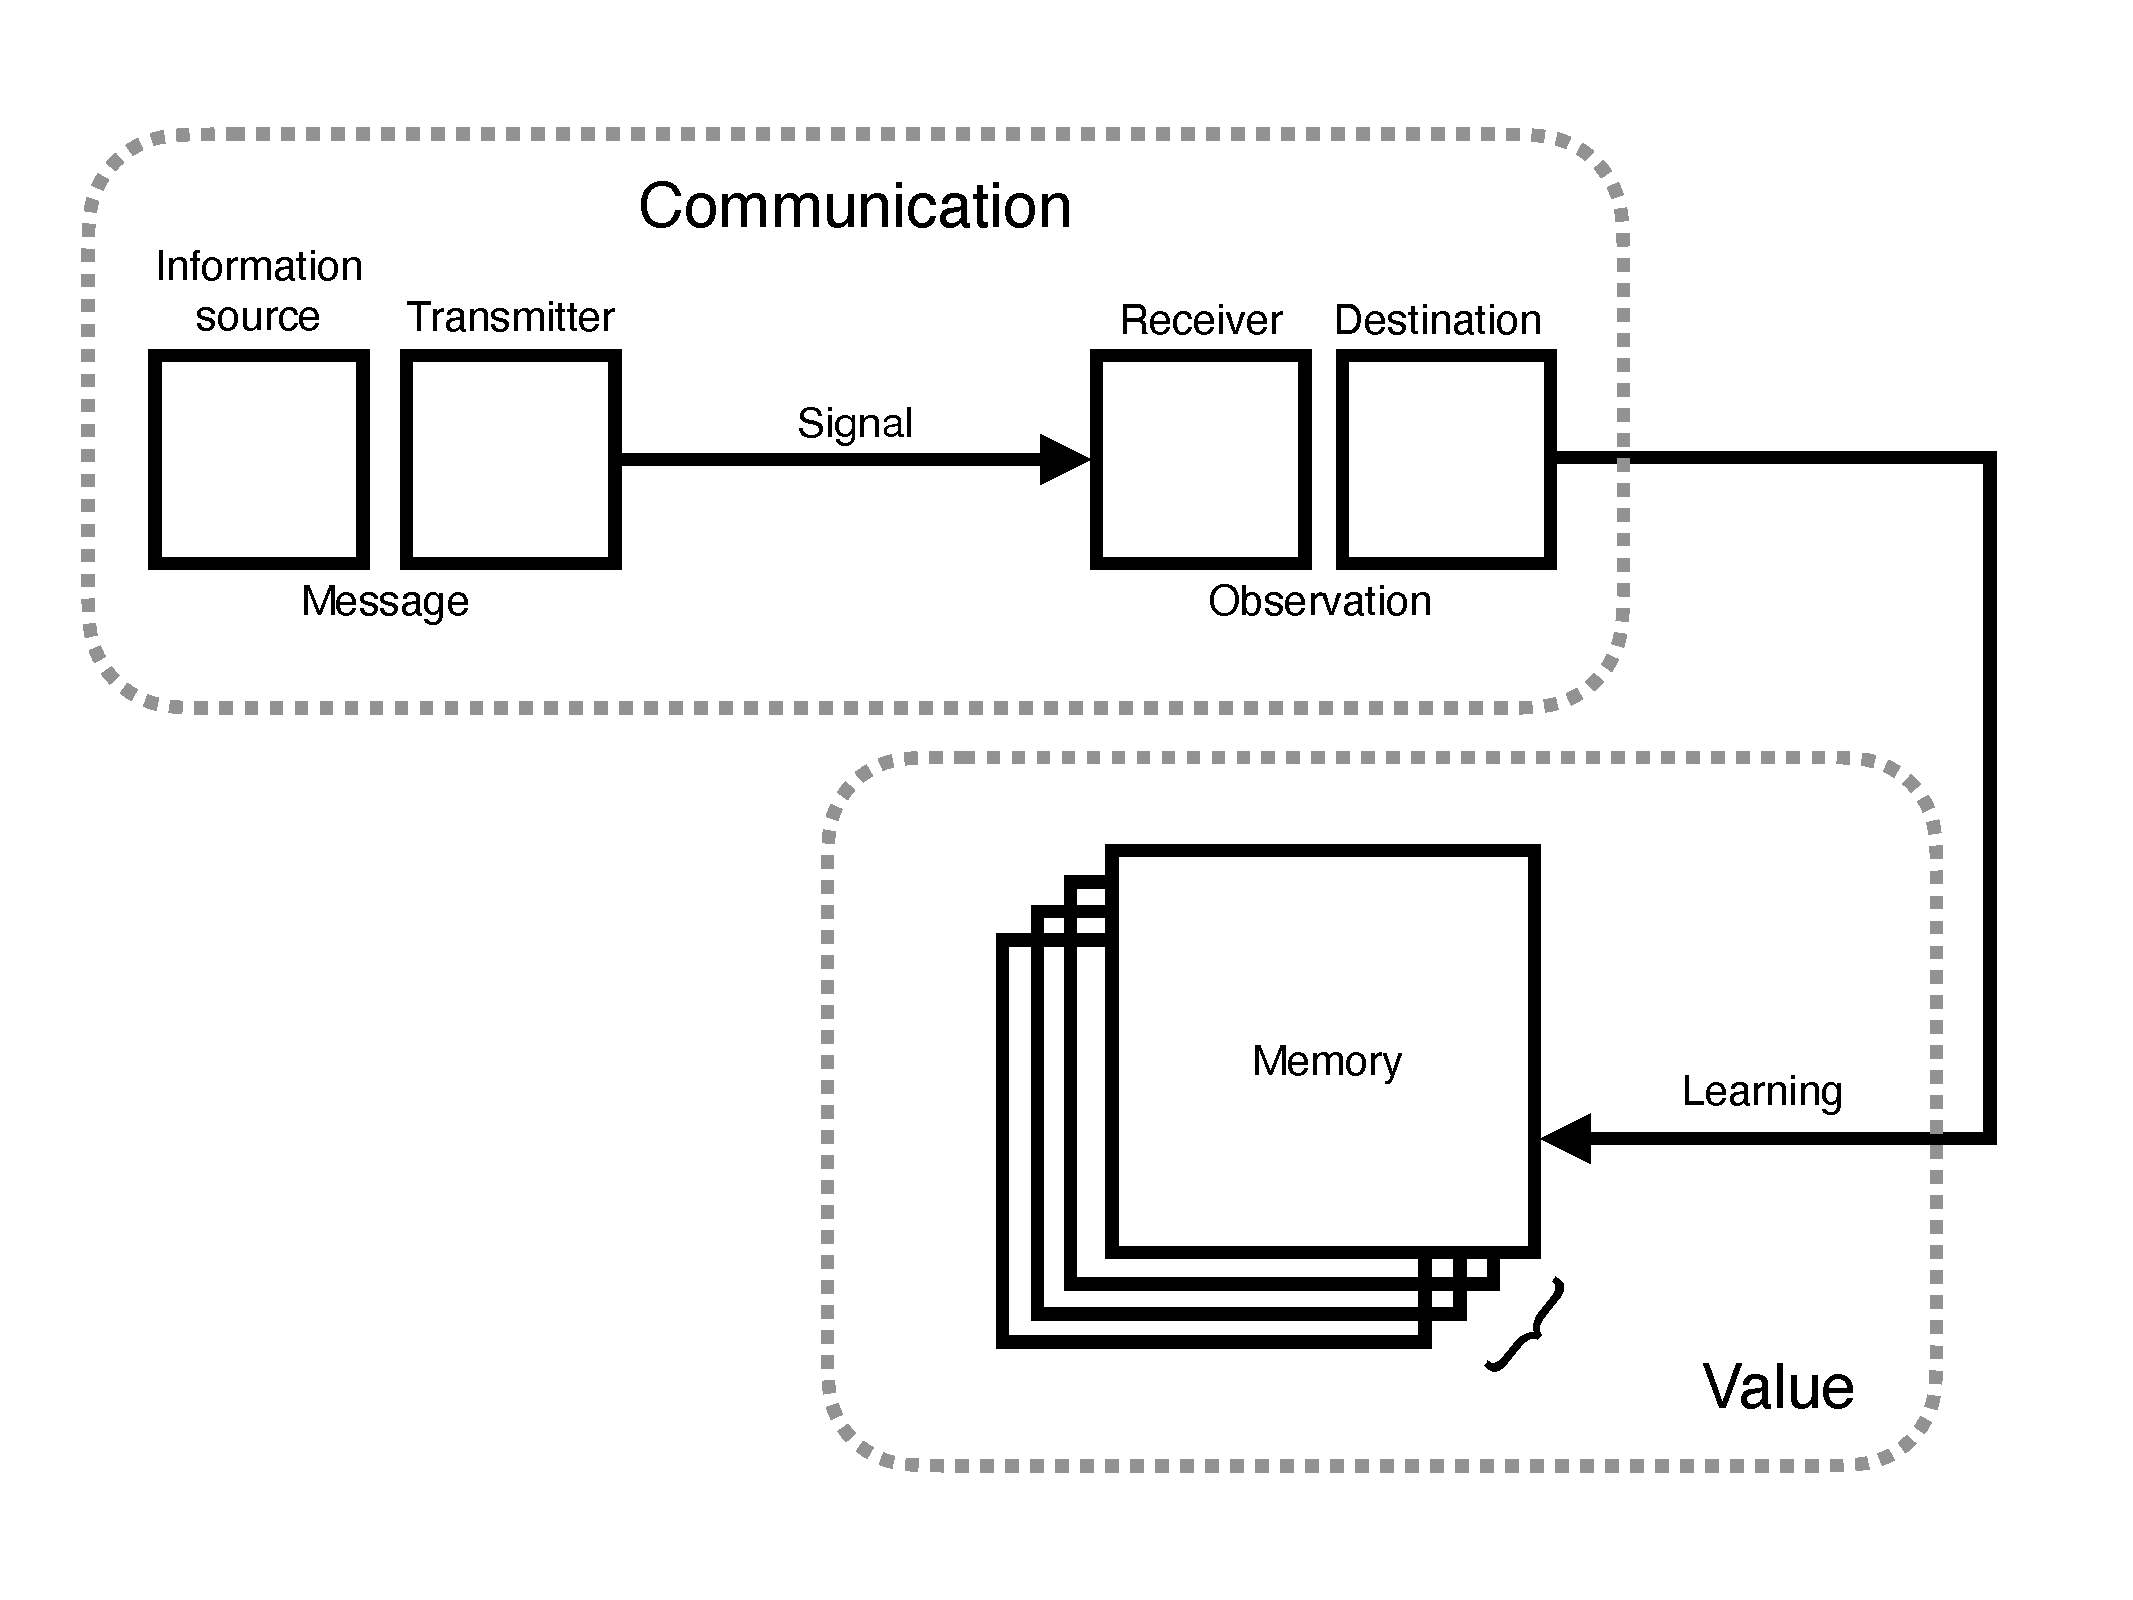
\includegraphics[width=0.7\linewidth]{img/info_diagram.pdf} 
    \caption{The relationship between the technical problem of communication with the technical problem of value. Note how value is not derived from the channel. Value is derived from learning about observations, which is in turn dependent on memory and its past history.
    }
    \label{fig:info1} 
\end{fullwidth}
\end{figure}

There is however an analogous set of levels for information value as to those Weaver describes. a. There is the technical problem of judging how much was learned. b. There is the semantic problem of both what this learning ``means'', and also what its consequences are. c. There is an effectiveness problem of using what was learned to some other effect. In many ways b and c are similar to those in the information theory. It is which is most different. 

For the same reasons Shannon avoided b and c in his theory, we have avoided them. Both of them are very hard to measure which makes them very hard to study mathematically. We fel it necessary to build a theory of information value which can act as a companion for information theory. This is why we took an axiomatic approach, and why we have tried to ape Shannon's axioms, as it made sense to do so.


\subsection(Does value as a technical problem even make sense?)
Information value has been taken up as a problem in meaning, or usefulness \cite{needed}. These are based on what we will call b-type questions (a notion we defined in the section above). It is not that b questions are not important or are not valuable. It is that they are second order questions. The first order questions are the 'technical' or a-type questions (also defined above). 

Having a technical definition for value, free from any meaning, might seem counterintuitive for a value measure. But we argue that it is not more or less counterintuitive than stripping information of meaning in the first  place. (This is how Shannon got his information theory). The central question for our account of value is, is it useful? It is enough to ensure a complete but perfectly efficient search for information/learning in any finite space. It is enough to play a critical part in solving/replacing the dilemma, which has for many years looked intractable. 


\subsection*{What about mutual information, or truth?}
In other prototypical examples, information value is based on how well what is learned relates to the environment \cite{needed}. Their mutual information that is. (Colloquially, one might call this truth.) The larger the mutual information between the environment and the memory, the more value it is said that we should then expect. This view seems to us at odds with actual learning behavior, especially in humans. 

As a people we pursue information which is fictional, or based on analogy, or outright wrong. Conspiracy theories, disinformation, and our many more mundane errors, are far too commonplace for value to be based on fidelity alone. This does not mean that holding false beliefs cannot harm survival. But this is a second order question as far as learning behavior foes. The fact that humans consistently seek to learn false things calls out that learning alone is a motivation. This is what opens the door for a technical definition.


\subsection*{So you suppose there is always positive value for learning of all fictions, disinformationist, and deceptions?}
This is our most unexpected prediction: We must.


\subsection*{What about information foraging?}
Our work is heavily inspired by information foraging. (We are also aware of its limits \cite{needed}). Our motivation in developing was that information value should not depend on only a probabilistic reasoning, as it does in information foraging. This is for the simple reason that many of the problems animals need to learn are not probabilistic problems \textit{from their point of view}. (Most any learning problem can be described as probabilistic from an outsider's perspective; the one scientists' rely on). We also felt the algorithmic curiosity looked so important that it needed as general a way to study it, which is why we developed an axiomatic approach that ended up addressing the technical problem of information value.


\subsection*{Was it necessary to build a general theory for information value just to describe curiosity?}
No. It was an idealistic choice, which worked out. The field of curiosity studies has shown there are many kinds of curiosity. At the extreme limit of this diversity is a notion of curiosity defined for any kind of observation, and any kind of learning. If we were able to develop a theory of value driven search at this limit, we can be sure it will apply in all possible examples of curiosity that we seem sure to discover in future. At this limit we can also be sure the ideas will span fields, addressing the problem as it appears in computer science, psychology, neuroscience, biology, and perhaps economics.


\subsection{Doesn't your definition of regret ignore lost rewards when the curiosity policy is in control?}
Yes. Regret is calculated for the policy which is in control of behavior, not the policy which \textit{could} have been in control of behavior.


\subsection*{Is information a reward?}
It depends. If reward is defined as more-or-less any quantity that motivates behavior, then our definition of information value is a reward. This does not mean however that information value and environmental rewards are interchangeable. In particular, if you add reward value and information value to motivate search you can drive exploration in practical and useful ways. But this doesn't change the intractability of the dilemma proper \cite{Thrun1992a,Dayan1996,Findling2018,Gershman2018b}. So exploration will still generate substantial regret (as we show in Fig \ref{fig:summary}). But perhaps more important is that these kinds of intrinsic rewards \cite{Schmidhuber1991,Berger-Tal2014,Itti2009,Friston2016,Kobayashi2019} introduce a bias that will drive behavior away from what, could otherwise be, ideal skill learning \cite{Ng1999,Simsek2006}.


\subsection*{Animal behavior and neural circuits}
In psychology and neuroscience, curiosity and reinforcement learning have developed as separate disciplines \cite{Berlyne1950,Kidd2015,Sutton2018}. And er hghilighted how they are separate problems, with links to different basic needs: gathering resources to maintain physiological homeostasis \cite{Keramati2014,Juechems2019} and gathering information to decide what to learn and to plan for the future \cite{Valiant1984,Sutton2018}. Here we suggest that though they are separate problems, they are problems that can, in large part, solve one another. This insight is the central idea to our view of the explore-exploit decisions. We'll now review evidence that evolution has respected this distinction. 

Cisek (2019) has traced the evolution of perception, cognition, and action circuits from the Metazoan to the modern age \cite{Cisek2019}. The circuits for reward exploitation and observation-driven exploration appear to have evolved separately, and act competitively--exactly the model we suggest. In particular he notes that exploration circuits in early animals were closely tied to the primary sense organs (i.e. information) and, historically anyway, had no input from the homeostatic circuits needed for reward valuation \cite{Keramati2014,Cisek2019,Juechems2019}. This neural separation for independent circuits has been observed in ``modern'' high animals, including zebrafish \cite{needed}, mouse \cite{needed}, humans \cite{needed}, and monkey \cite{White2019,Wang2019}. It is difficult to know the exact objectives of these circuits, but their independence aof activity and independence during behavior suggests they are, by degrees, independent policies.


\subsection*{What about aversive values?}
We do not believe this is complete theory. For example, we do not account for any consequences of learning, or any other aversive events. The need to add 
% TODO...


\subsection*{Fitting deterministic models?}
The theoretical description of exploration in scientific settings is probabilistic \cite{Calhoun2014,Song2019a,Gershman2018b,Schulz2018a}. By definition probabilistic models can't make exact predictions of behavior, only statistical ones. Our approach is deterministic, and so does make exact predictions. Our theory predicts that it should be possible to guide exploration in real-time using, for example, optogenetic methods in neuroscience, or well timed stimulus manipulations in economics or other behavioral sciences. 

In species ranging from human to \textit{Caenorhabditis elegans}, there are hundreds perhaps thousands of exploration-exploitation experiments. Analysis of their behavior has generally been limited to distributions. A deterministic theory can, in principle, open up entirely new avenues for reanalysis by using our model to make exact predictions.

\textbf{TODO} - discuss practical fits:
\begin{enumerate}
    \item Burn in
    \item Population E0, and refinement, replicators?
    \item Data fusion (bayes methods for deterministic equations are legit)
\end{enumerate}


\subsection*{Does regret matter?}
Another way around the dilemma is to ignore regret. This is the domain of pure exploration methods, like the Gitten’s Index \cite{needed}, or PAC approaches \cite{Valiant1984}, or other bounded forms of reinforcement learning \cite{needed}. Pure random search is another useful example. Such methods can guarantee you find the best value, often in an unbiased way. They can in some cases do so with a bound on the number of actions needed. These methods do not consider regret or missed value encountered during search. Regret might not be important in some settings, but we expect that when time and resources are scarce minimizing regret must be a critical skill for survival.


\subsection*{Summary}
There will be certainly cases in an animal's life when their exploration must focus on reward. But even here the search for reward information alone will make the search more robust to deception, and more reliable in the future. Think of this as curiosity about reward. But there are many more cases where curiosity can include observations of the environment, and the self. This paper has argued that one should put aside intuitions which suggest open-ended curious search is too inefficient to be practical. We have shown how it can be made very practical. We have argued one should put aside intuitions for what exploration behavior represents, and used this to offer a zero-regret way around the dilemma -- a problem which has seemed unsolvable.



\section*{Acknowledgments}
We wish to thank Jack Burgess, Matt Clapp, Kyle ``Donovank'' Dunovan, Richard Gao, Roberta Klatzky, Jayanth Koushik, Alp Muyesser, Jonathan Rubin, and Rachel Storer for their comments on earlier drafts. We also wishes to thank Richard Grant for his illustration work in Figure 1, and Jack Burgess for his assitance with Figure~\ref{fig:task_outline}.

The research was sponsored by the Air Force Research Laboratory (AFRL/AFOSR) award FA9550-18-1-0251. The views and conclusions contained in this document are those of the authors and should not be interpreted as representing the official policies, either expressed or implied, of the Army Research Laboratory or the U.S. government. TV was supported by the Pennsylvania Department of Health Formula Award SAP4100062201, and National Science Foundation CAREER Award 1351748.

\bibliography{library,tim_refs} % TODO - fix me?

\newpage
\section*{Mathematical Appendix.}
\newcommand{\beginsupplement}{%
        \setcounter{table}{0}
        \renewcommand{\thetable}{S\arabic{table}}%
        \setcounter{figure}{0}
        \renewcommand{\thefigure}{S\arabic{figure}}%
     }
\beginsupplement
\setcounter{theorem}{0}

% --------------------------------------------------------------------------
\subsection*{Optimal substructure in memory}
To find an optimal value solution for $\hat E$ using the Bellman equation we must prove our memory $\mathbf{M}$ has optimal substructure. This is because the normal route, which assumes the problem rests in a Markov Space, is closed to us. By optimal substructure we mean that the process of learning in $\mathbf{M}$, and therefore maximization of $\hat E$ can be partitioned into a collection, or series of memories, each of which is itself an max value solution.

This opaque term of optimal substructure can be intuitivily understood by looking in turn at another theoretical construct, Markov spaces. 

In Markov spaces there are a set of states $(S_0, S_1, \ldots)$, where the transition to the next $S_t$ depends only on the previous state $S_{t-1}$. This limit means that if we were to optimize over these states, as in reinforcement learning, we know that we can treat each transition as its own ``subproblem'', and ignore the history's $(S_0, S_1, \ldots)$ effect on value, and therefore the overall situation has ``optimal substructure''.

The problem for our defintion of information value is it relies on memory which is necessarily composed of many past observations, in many orders, and so it cannot be a Markov space. So if we wish to use the Bellman equation, we need to find another way to establish optimal substructure. This is the focus of Theorem~\ref{theorem:opt_sub}. In this theorem we implicitly assume that $\mathbf{X} = \mathbf{S}$, $\mathbf{A}$, $\mathbf{M}$, $f$, and $\Lambda$ are given, and that $\Lambda$ is deterministic, 

\begin{theorem}[Optimal substructure] \label{theorem:opt_sub} 
   If $V^*_{\pi_{\hat E}}$ is the optimal information value given by policy $\pi_{\hat E}$, a memory $\mathbf{M}_t$ has optimal substructure if the last observation $X$ can be removed from $\mathbf{M}$, by $\mathbf{M-1}_{t} = f^{-1}(\mathbf{X}, \mathbf{M}_t)$ such that the resulting value $V^*_{t-1} = V^*_{t} - E_{t}$ is also optimal. 
\end{theorem}
\begin{proof}
	Given a known optimal value $V^*$ given by $\pi_{\hat E}$ we assume for the sake of contradiction there also exists an alternative policy $\hat \pi_{\hat E} \neq \pi_{\hat E}$ that gives a memory $\hat{\mathbf{M}}_{t-1} \neq \mathbf{M}_{t-1}$ and for which $\hat V^*_{t-1} > V^*_{t-1}$. 
	
	To recover the known optimal memory $\mathbf{M}_t$ we lift $\hat{\mathbf{M}}_{t-1}$ to $\mathbf{M}_t = f(\hat{\mathbf{M}}_{t-1}, \mathbf{X}_t)$. This implies $\hat V^* > V^*$ which in turn contradicts the purported original optimality of $V^*$ and therefore $\hat \pi_{\hat E}$.
\end{proof}

This proof requires two things. First, we need to a mechanism of forgetting, of a very particular kind. We assume that the last learning step $f(\mathbf{X}, \mathbf{M}) \rightarrow \mathbf{M}'$ can be undone by a new vector valued function $f^{-1}$, such that $f(\mathbf{X}, \mathbf{M'}) \rightarrow \mathbf{M}$. In other words we must assume what was last remembered, can always be exactly forgotten. Second, we assume the environmental dynamics, given by the transition function $\Lambda$, are deterministic. 

Determinism is consistent with the natural world which does evolve in a deterministic way, at the scale of animal behavoir that we concerned with at least. This assumption is however at odds with much of reinforcement learning theory \cite{Sutton2018} and past experimental work. For example, \cite{Gershman2018}. Both tend to study stochastic environments. We addressed this discrepancy in the main text, using numerical simulations.


% ------------------------------------------------------------------------
\subsection*{Bellman optimal information collection}
We aim to find a series of actions $(\mathbf{A}_1, \mathbf{A}_2, ..\mathbf{A}_T)$, drawn from a set $\mathbb{A}$, that maximize each payout $(\hat E_0, \hat E_1, \ldots, \hat E_{T})$ so the total payout received is as large as possible. If there is a policy $\mathbf{A} = \pi(\mathbf{X})$ to take actions, based on a series of observations $(X_0, X_1, ..X_{T}),$, given by $\Lambda$, then an optimal policy $\pi^*$ will always find the maximum total value $V^* = \argmax_{\mathbf{A} \in \mathbb{A}} \sum_T \hat E_t $. In the form above one would need to reconsider the entire sequence of actions for any one change to that sequence, leading to a combinatorial explosion. Bellman's insight was a way to make this last problem simpler by breaking it down into a small set of subproblems that we can solve in a tractable way without an explosion in complexity. This is his principle of optimality, which reads:

\begin{quote}
    An optimal policy has the property that whatever the initial state and initial decision are, the remaining decisions must constitute an optimal policy with regard to the state resulting from the first decision. \cite{Bellmann1954}
\end{quote}

Mathematically Bellman's principle allows us to translate the full problem, $V^* = \argmax_{\pi} \sum_T \hat E_1, \hat E_2, ..., \hat E_{T}$ to a recursive one. Having already proven the optimal substructure of $\mathbf{M}$, and given an arbitrary starting value $E_0$, the Bellman solution to curiosity optimization of $\hat E$ is therefore given by,

\begin{equation} 
	\label{eq:bellman_iter_E_app}
	V^*_{\hat E}(\mathbf{S}) = \argmax_{\mathbf{A} \in \mathbb{A}} \Big [ \hat E_{t}  + V^*_{\hat E}(\Lambda(\mathbf{S},\mathbf{A})) \Big ]
\end{equation}


% ------------------------------------------------------------------------
\subsection*{Optimal exploration} 

Recall from the main text we consider that a good exploration should,

\begin{enumerate}
	\item Exploration should visit all available states of the environment at least once.
	\item Exploration should cease when learning has plateaued.
	\item Exploration should take as few steps as possible to achieve 1 and 2.
\end{enumerate}

If $\pi_{\hat E}$ to a deterministic policy this makes proving these three properties amounts to solving sorting problems on $\hat E$, and assuming $\mathbf{X} = \mathbf{S}$. That is, if a state is visited by our algorithm it must have the highest value, by definition. So if every state must be visited every state must, at one time or another, give the maximum value. This is certain to happend if we know that all values will begin contracting towards zero, in finite time. 

\textbf{Definitions.} Let $\mathbb{Z}$ be the set of all visited states, where $\mathbb{Z}_0$ is the empty set $\{\}$ and $\mathbb{Z}$ is built iteratively over a path $P$, such that $\mathbb{Z} \rightarrow \{\mathbf{S} | \mathbf{S} \in \mathbb{S}\ \text{and}\ x \not\in \mathbf{Z}\}$. 

To formalize the idea of ranking we take an algebraic approach. Give any three real numbers $(a,b,c)$,

\begin{align}\label{eq:ineq} 
	a \leq b \Leftrightarrow \exists \ c;\ b = a + c \\
	a > b \Leftrightarrow (a \neq b) \wedge (b \leq a) 
\end{align}

\begin{theorem}[Complete exploration] \label{theorem:Z} 
	Given some arbitrary value $\hat E_0$, an exploration policy governed by $\pi_{\hat E}$ will visit all states $\mathbf{S} \in \mathbb{S}$ in finite number of steps $T$.
\end{theorem}
\begin{proof}
	Let $\mathbf{E} = (\hat E_1, \hat E_2, ...)$ be ranked series of $\hat E$ values for all states $\mathbf{S}$, such that $(\hat E_1 \geq \hat E_2, \geq ...)$. To swap any pair of values ($\hat E_i \geq \hat E_j$) so ($\hat E_i \leq \hat E_j$) by Eq.~\ref{eq:ineq} $\hat E_i - c = \hat E_j$. 
	
	Therefore, again by Eq.~\ref{eq:ineq}, $\exists \int \delta \hat E \rightarrow -c$. 
	
	\textit{Recall}: Axiom 4 - $\nabla^2 \mathbf{M} < 0$ after a finite time $T^*$.
	
	However if we wished to instead swap ($\hat E_i \leq \hat E_j$) so ($\hat E_i \geq \hat E_j$) by definition $\not \exists c; \hat E_i + c = \hat E_j$, as $\not \exists \int \delta \hat E \rightarrow c$. 
	
	To complete the proof, assume that some policy $\hat \pi_{\hat E} \neq \pi^*_E$. By definition policy $\hat \pi_{\hat E}$ can be any action but the maximum, leaving $k-1$ options. Eventually as $t \rightarrow T*$ the only possible swap is between the max option and the $kth$, but as we have already proven this is impossible as long as Axiom 4 holds. Therefore, the policy $\hat \pi_{\hat E}$ will leave at least 1 option unexplored and $S \neq Z$. 
\end{proof}

\begin{theorem}[[Efficient exploration] \label{theorem:convergence} 
	An exploration policy governed by $\pi^*_{\hat E}$ will revisit all states in exact proption to their information value.
\end{theorem}
\begin{proof}
    \textit{Recall}: Theorem~\ref{theorem:Z}.
    \textit{Recall}: $\pi^*_E$ is a maximum value deterministic algorithm.
	\textit{Recall}: Axiom 2. Each time $\pi^*_E$ visits a state $\mathbf{S}$, so $\mathbf{M} \rightarrow \mathbf{M}'$, and after $T^*$ it is axiomatically true $\hat{E}' < \hat E$
	
	By induction then, if $\pi^*E$ will visit all $\mathbf{S} \in \mathbb{S}$ in $T^*$ trials, it will revisit them at most $2T^*$, therefore as $t \rightarrow \infty$, $E \rightarrow \eta$, where $eta > 0$. 
\end{proof}

These exploration proofs come with some fine print, for practical work. $E_0$ can be any positive and finite real number, $E_0 > 0$. Different choices for $E_0$ will not change the proofs, especially their convergence. So in that sense one can chosen it in an arbitrary way. Different choices for $E_0$ can however change individual choices, and their order. This can be quite important in practice, especially when trying to describe some real data.  

% ---------------------------------------------------------------------------------
\subsection*{Optimality of $\Pi_{\pi}$} 
Recall that in the main text we introduce the equation below as a candidate with zero regret solution to exploration-exploitation problems, set in terms the mixed value sequence $V_{\hat{E}R}$.

\begin{equation} 
    \label{eq:pipi_app}
    \begin{split}
        \Pi_{\pi} = 
        \begin{cases}
            \pi^*_{\hat{E}} & : \hat{E} - \eta > R + \rho \\
            \pi_R 	& : \hat{E} - \eta < R + \rho \\
        \end{cases}
    \end{split}
\end{equation}

In the following section we prove two things about the optimality of $\pi_\pi$. First, if $\pi_R$ had any optimal asymptotic property for value learning before their inclusion into our scheduler, they retain that optimal property under $\pi_\pi$ when $\eta = 0$, or is otherwise sufficiently small. Second, show that if both $\pi_R$ and $\pi_E$ are greedy, and $\pi_\pi$ is greedy in its definition, then Eq~\ref{eq:pipi} is certain to maximize total value. The total value of $R$ and $\hat E$ is the exact quantity to maximize if information seeking and reward seeking are equally important, overall. This is, as the reader may recall, one of our key assumptions. Proving this optimality is analogous to the classic activity selection problem from the job scheduling literature \cite{BellmanBook,Roughgarden2019}.

\begin{theorem}[$\pi_{\pi}$ is unbiased] \label{theorem:meta} 
	 Let any $S$, $\mathbf{A}$, $\mathbf{M}$, $\pi_R$, $\pi_E$, and $\delta$ be given. Assuming an infinite time horizon, if $\pi_E$ is optimal and $\pi_R$ is optimal, then $\pi_{\pi}$ is also optimal in the same sense as $\pi_E$ and $\pi_R$. 
\end{theorem}
\begin{proof}
	The optimality of $\pi_{\pi}$ can be seen by direct inspection. If $p(R = 0) > 0$ we are given an infinite horizon, then $\pi_E$ will have a unbounded number of trials meaning the optimally of $P^*$ holds. Likewise, $\sum E < \eta$ as $T \rightarrow \infty$, ensuring $pi_R$ will dominate $\pi_{\pi}$ therefore $\pi_R$ will asymptotically converge to optimal behavior. 
\end{proof}

In proving this optimality of $\pi_{\pi}$ we limit the probability of a positive reward to less than one, denoted by $p(R_t = 1) < 1$. Without this constraint the reward policy $\pi_R$ would always dominate $\pi_{\pi}$ when rewards are certain. While this might be useful in some circumstances, from the point of view $\pi_E$ it is extremely suboptimal. The model would never explore. Limiting $p(R_t = 1) < 1$ is a reasonable constraint, as rewards in the real world are rarely certain. A more naturalistic way to handle this edge case is to introduce reward satiety, or a model physiological homeostasis \cite{Keramati2014,Juechems2019}.

In classic scheduling problems the value of any job is known ahead of time \cite{Bellmann1954,Roughgarden2019}. In our setting, this is not true. Reward value is generated by the environment, \textit{after} taking an action. In a similar vein, information value can only be calculated \textit{after} observing a new state. Yet Eq.~\ref{eq:pipi} must make decisions \textit{before} taking an action. If we had a perfect model of the environment, then we could predict these future values accurately with model-based control. In the general case though we don't know what environment to expect, let alone having a perfect model of it. As a result, we make a worst-case assumption: the environment can arbitrarily change--bifurcate--at any time. This is a highly nonlinear dynamical system \cite{Strogatz1994}. In such systems, myopic control--using only the most recent value to predict the next value-- is known to be an robust and efficient form of control \cite{Hocker2019}. We therefore assume that last value is the best predictor of the next value, and use this assumption along with Theorem~\ref{theorem:meta} to complete a trivial proof that Eq.~\ref{eq:pipi} maximizes total value.

\subsubsection*{A win-stay, lose-switch solution}
If we prove $\pi_{\pi}$ has optimal substructure, then using the same replacement argument \cite{Roughgarden2019} as in Theorem~\ref{theorem:meta}, a greedy policy for $\pi_\pi$ will maximize total value.

\begin{theorem}[No regret - mixed values]
	\label{th:no_regret_ER}
	When either $\pi_{\hat E}$ or $\pi_R$ is in control under $\Pi_{\pi}$, all actions are zero regret in terms of $V_{\hat{E}R}$. That is, $\sum_{k=0}^{T} G = 0$.
\end{theorem}

% HERE- TODO - this should be a simple substitution proof.

% \begin{theorem}[Total value maximization of $\pi_{\pi}$] \label{theorem:metA_total} 
%     \label{theorem:meta} 
% 	 Let any $S$, $A$, $\mathbf{M}$, $\pi_R$, and $\delta$ be given. If $\pi_R$ is defined on a Markov Decisions, then $\pi_\pi$ is Bellman optimal and will maximize total value. 
% \end{theorem}
% \begin{proof}
%     We assume Reinforcement learning algorithms are embedded in Markov Decisions space, which by definition has the same decomposition properties as that found in optimal substructure.
    
%     \textit{Recall}: The memory $\mathbf{M}$ has optimal substructure (Theorem~\ref{theorem:opt_sub}.
    
% 	\textit{Recall}: The asymptotic behavior of $\pi_R$ and $\pi_E$ are independent under $\pi_\pi$ (Theorem~\ref{theorem:meta}
	
% 	\textit{Recall}: The controller $\Pi_\pi$ is deterministic.
	
% 	If both $\pi_R$ and $\pi_E$ have optimal substructure independently, and are independent under $\Pi_\pi$, then $\Pi_\pi$ must also have optimal substructure. If $\pi_\pi$ has optimal substructure, then it is Bellman optimal.
% \end{proof}


% --------------------------------------------------------------------
\end{document}


